\documentclass[12pt]{article}
\usepackage[margin=1in]{geometry}
\setlength\parindent{0pt}
\usepackage{amsmath,amssymb}
\usepackage{graphicx}
\usepackage{endnotes}
\let\footnote=\endnote
\renewcommand{\notesname}{Works Cited}
\usepackage{float}
\usepackage{hyperref}
\usepackage{xurl}
\hypersetup{
    colorlinks=true,
    linkcolor=blue,
    filecolor=magenta,      
    urlcolor=blue,
}
\usepackage{subfigure}
\usepackage{caption}
\usepackage{subcaption}
\captionsetup[figure]{font=small}
\usepackage{setspace}
\linespread{1.5}
\title{PPOL564 Final Project: Predicting Election Results}
\author{Colette Yeager}
\date{Word Count: 2992}
\begin{document}
\maketitle

\section*{Introduction}

For this project, I chose to look at all of the features that play a role in the results of presidential elections, to see which are the most influential. In this report, I will show how I pull data from several different sources to see election results, economic growth, state results, turnout rates, and information about each president. I will go through the process of how I organized, cleaned, and combined my data to end up with a τοταλ data set and database to be able to model. Ultimately, the statistical model I am looking at is how each of these factors predict a President's winning vote share. I will then look at some of my results from the statistical models and analyze which features ended up being the best predictors.

\section*{Problem Statement and Background}

The goal of my project was to determine which factors are most important in predicting future election results. There have been many studies related to this topic, both by campaigns and forecasters such as those at FiveThirtyEight. Doing these types of studies can very helpful in determining the best campaigning strategies. These studies focus mostly on results from polls\footnote[1]{Graefe, Andreas. "Predicting Elections: Experts, Polls, and Fundamentals." Judgment and Decision Making, vol. 13, no. 4, July 2018, pp. 334-44, \url{www.sas.upenn.edu/~baron/journal/18/18124/jdm18124.pdf}.}; I wanted to see if I could find other key useful predictors other than this. 

\vspace{3.00mm}

One famous system for predicting outcome is The Keys to the White House, a checklist of 13 statements about the circumstances surrounding a presidential election\footnote[2]{"Keys to the White House." PollyVote, \url{pollyvote.com/en/components/models/mixed/keys-to-the-white-house/}.}. Many of these are difficult to measure quantitatively, such as whether there was social unrest during the previous term or whether the candidate is charismatic or a national hero. Two that I decided to use in similar ways in my study were whether the incumbent-party candidate is the sitting president and the level of economic growth in the previous term. 

\vspace{3.00mm}

Economic growth in particular has been widely studied over the world, especially when one of the candidates is the incumbent. When the economy has not grown or gotten worse during an administration, voters might be likely to vote for the party or same person that was in office previously. One discussion shows that the extent that economic performance is reflected in vote share is reflected by citizen's evaluations of the overall economy\footnote[3]{Becher, Michael, and Michael Donnelly. "Economic Performance, Individual Evaluations, and the Vote: Investigating the Causal Mechanism." The Journal of Politics, vol. 75, no. 4, 2013. Chicago Journals, \url{https://doi.org/10.1017/S0022381613000959}.}. In this study, they similarly pulled from several years of elections, and used results from many countries to make their analysis. 

\vspace{3.00mm}

While there are certainly many other factors that play similar roles, such as some discussed in the above studies, I wanted to use a larger variety of predictors, and focus on key ones from multiple categories of factors, rather than every possible measure. Turnout is a more general factor that has a variety of effects on election results. Originally, when I began this project, I wanted to look at turnout from the primary election by party, and compare this to the vote share and winning party. However, this became too difficult to obtain, so I used overall turnout, which still had an effect on vote share, as seen below in my analysis. 

\vspace{3.00mm}

I also chose to look at some results from key states as a slightly separate section of this study. I was interested to see if I could determine which states are the most predictive of election results based on previous voting patterns. This would be helpful for campaigns, as they would want to spend the most amount of time talking with voters from the states that play the biggest role in determining election results.

\vspace{3.00mm}

I had to make some assumptions going into the project to make my data and analysis a little simpler. First, in comparing the political party of the Presidential candidate to that of the previous President and whether or not the candidate was an incumbent, I removed all the Presidents that didn't come into office through an election. This means that some of the points where I assess whether a President had the same party as the previous President are incorrect, but there are not too many, and it would have been significantly more difficult to find the true results. Additionally, in calculating swing states for comparison, I measured which states have been the most accurate over time, even though they might not accurately reflect the states considered to be swing states today. I discuss this further in the analysis section. 

\section*{Data}

\subsection*{Election Results}

The first dataset that I pulled was a history of election results since the first presidential "election" in 1789. This data came from Statista\footnote[4]{O'Neill, Aaron. "Share of Electoral and Popular Votes by Each United States President 1789-2020." Statista, 18 Feb. 2021, \url{www.statista.com/statistics/1034688/share-electoral-popular-votes-each-president-since-1789/}.} in a downloadable form, so I was able to just use the \verb|read_excel| function to read in this data. This data was relatively tidy - I split up the column that contained both the President name and year into two columns, took out the percentage signs from the Vote Share columns, and made sure the Year and Vote Share columns were all treated as integers and floats. These Vote Share results would then be treated as my dependent variable.

\subsection*{Previous Presidents}

My next dataset was pulled from Wikipedia\footnote[5]{"List of Presidents of the United States." Wikipedia, \url{en.wikipedia.org/wiki/List_of_presidents_of_the_United_States}.}, so I was able to use the \verb|read_html| package to scrape the table, which included factors about each President. The elements that I ultimately ended up including were Year, Name, and Party, which I was then able to transform later on to analyze whether the previous President was the same President running and whether the previous President had the same party. To clean this data, I created a function to change the political party name to a shorter version to match that in the state results data. To get rid of Presidents that hadn't been elected into office, I dropped all duplicates by Election Year, and also had to drop duplicates by Name and Election Year to get rid of rows where the President changed party midway through their term. For simplicity, I kept their first party.

\subsection*{Economic Growth}

I pulled data on economic growth from Statista\footnote[6]{O'Neill, Aaron. "Annual GDP Growth for the United States 1930-2020." Statista, 29 Nov. 2021, \url{www.statista.com/statistics/996758/rea-gdp-growth-united-states-1930-2019/}.}, so used \verb|read_excel| after downloading. This data was for every year since 1932, not just the presidential years, so I selected the election years by only including years that were divisible by 4. 

\subsection*{State Votes}

For data on which party each state has voted for, I used \verb|read_html| to pull from Wikipedia\footnote[7]{"List of United States Presidential Election Results by State." Wikipedia, \url{en.wikipedia.org/wiki/List_of_United_States_presidential_election_results_by_state}.}. This included some additional label columns and rows, which I dropped, and then transposed to have a column for Year and columns for each state. Then, I merged the party column from the Presidential data into this dataset to be able to compare the party each state voted for with the party of the winning President. I then wanted to determine which states were the most accurate - i.e., which states had voted with the winning party the largest number of times. This would give me a general sense of which states, over time, could be the most predictive of a party winning. I calculated overall accuracy by summing the number of times a state voted for the winning party and dividing by the total number of times a state has been able to vote. I found that New Mexico, Illinois, Ohio, California, Pennsylvania, New York, and Nevada has the highest overall accuracy. 

\vspace{3.00mm}

I calculated this a second time as well, this time weighting the 8 most recent elections as 10 times higher to account for the fact that some states began voting a certain way in more recent years. From this, I found that Ohio, Nevada, Pennsylvania, New Mexico, Wisconsin, New Hampshire, and Michigan could be seen as the most accurate current swing states. I then added all of the states, both overall and current to a new data frame as dummy variables, where the value was 1 if in a given year the state voted for the winning party.

\subsection*{Turnout}

Finally, I pulled data on turnout from each year, using \verb|read_html| again\footnote[8]{"National General Election VEP Turnout Rates, 1789-Present." United States Elections Project, \url{www.electproject.org/national-1789-present}.}. This data was only through 2016, so I manually found the turnout rate from 2020 and added it into the dataset.

\subsection*{Total Dataset}

After all of my data had been pulled and organized, I merged them into one larger data frame. For combining the information on previous Presidents, I had to add a current year column to the previous Presidents data frame, as Year + 4, and then merged based on this new column. Finally, I created some new columns with dummy variables for incumbent status and whether the candidate was the same party as the previous President. In the end, I stored all of these datasets into a SQL database so that I would be able to access them in multiple files.

\section*{Analysis}

Looking at the data, you can see that there are some missing values from the Popular Vote and Change in GDP columns:

\begin{figure}[H]
    \centering
    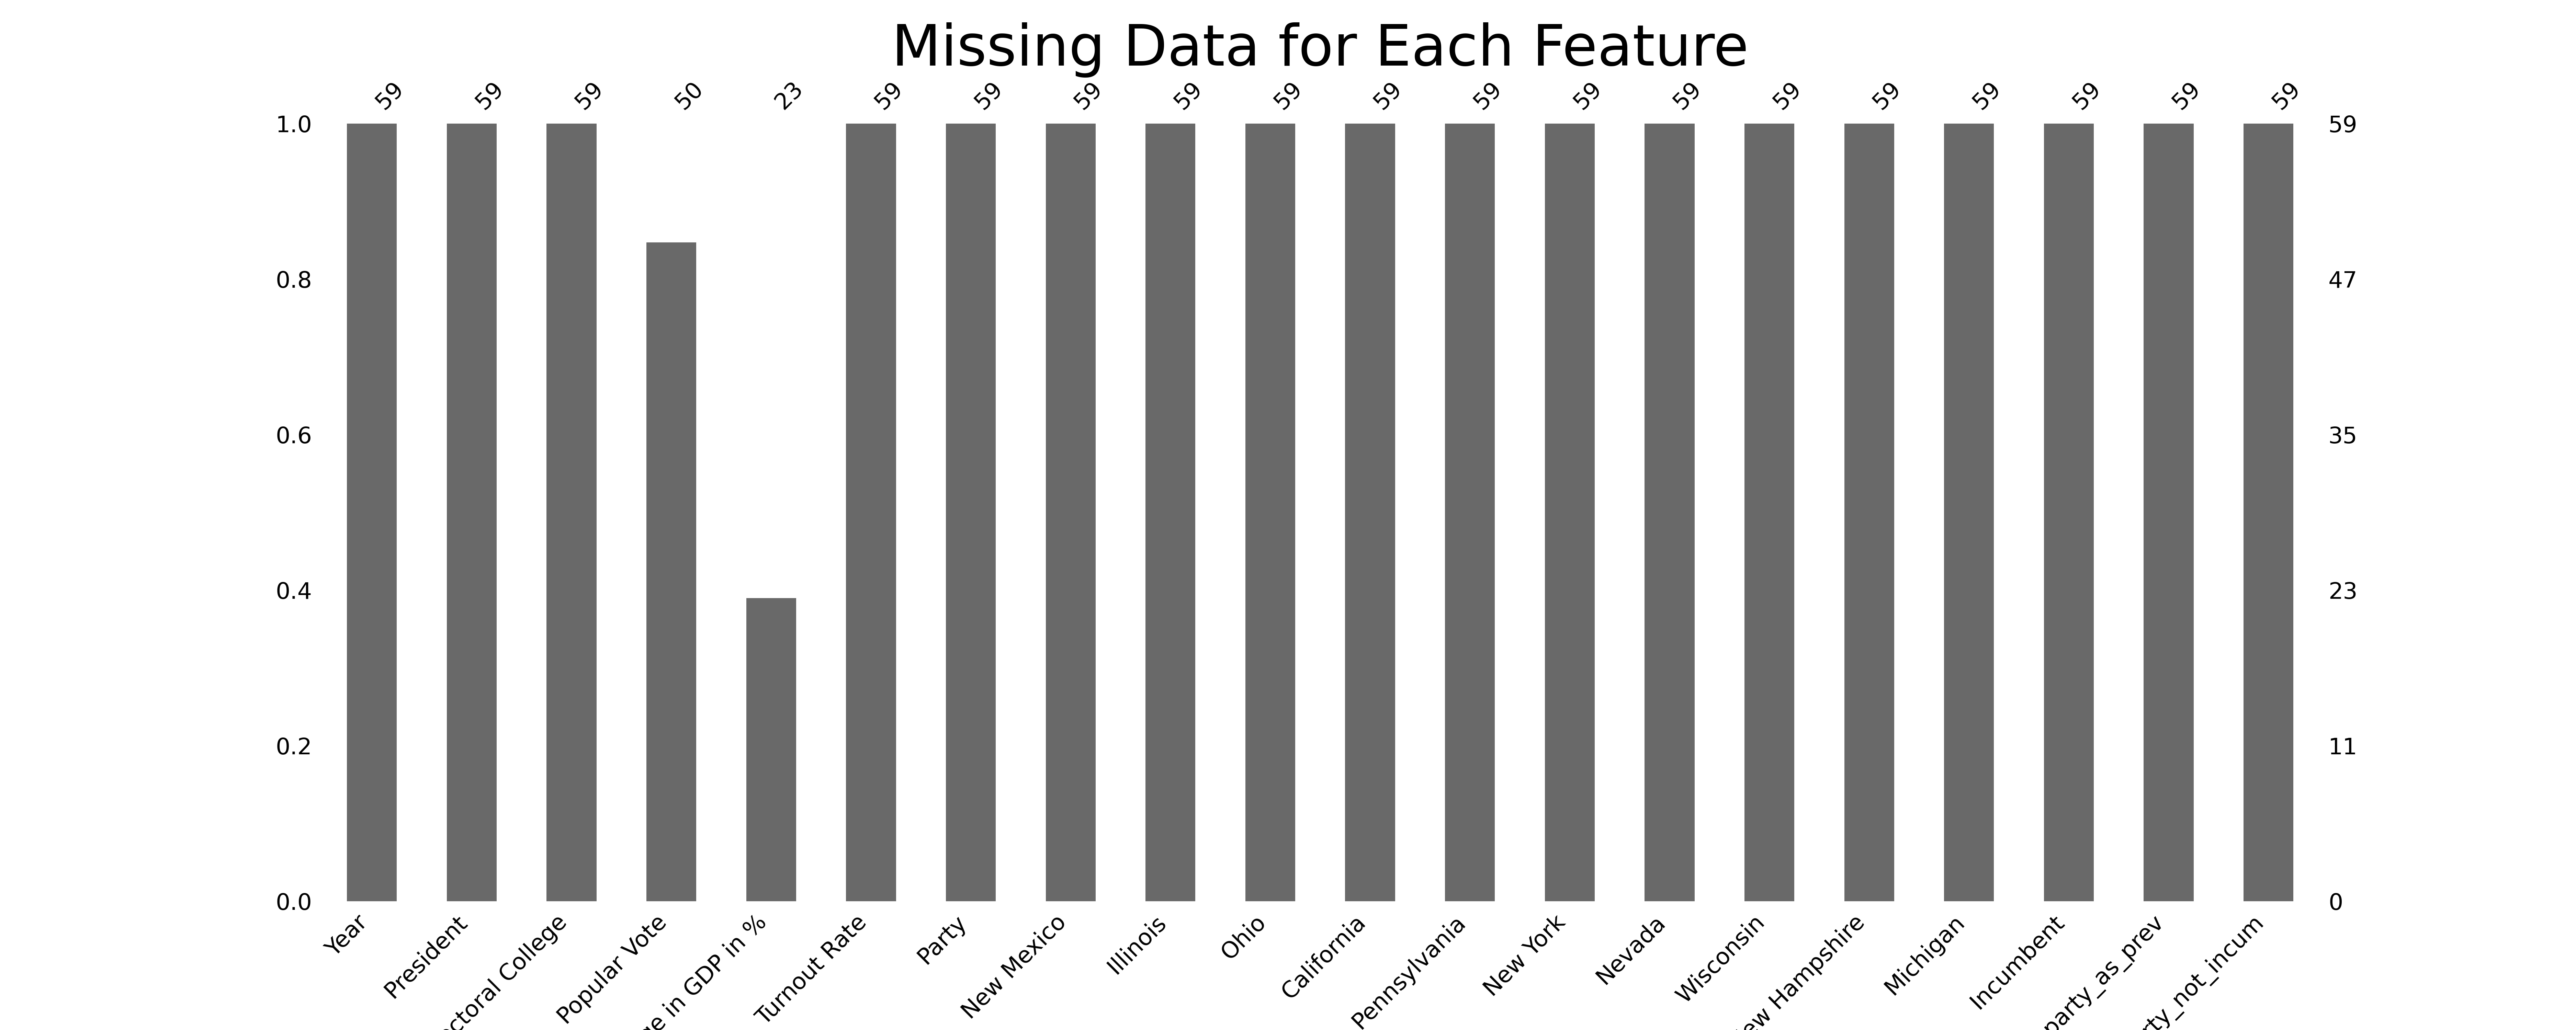
\includegraphics[width=0.9\linewidth]{Missing_Data.png}
    \caption{Missing Data}
\end{figure}

This is the case as these two features weren't measured until a certain point in time. Since these two variables were important to my analysis, I didn't want to get rid of them, but also didn't want to only look at rows that had all data present. Therefore, I decided to create a couple different versions of my data and compare results of my models. First, I created a subset that excluded the GDP variable. In general, I used vote share as my dependent variable, but switched off between using Electoral College and Popular Vote as I wanted to be able to look at them both individually. In my opinion, Popular Vote is a better measure of vote share in this situation as it more closely reflects the patterns and decisions of the actual voters, which ties in more closely to my independent variables. However, this wasn't measured until 1824, so I wanted to look at Electoral College as well to have more data points for my assessment. You can see from Figure 2 below that there were some differences in the trends between the two measures of vote share.

\begin{figure}[H]
    \centering
    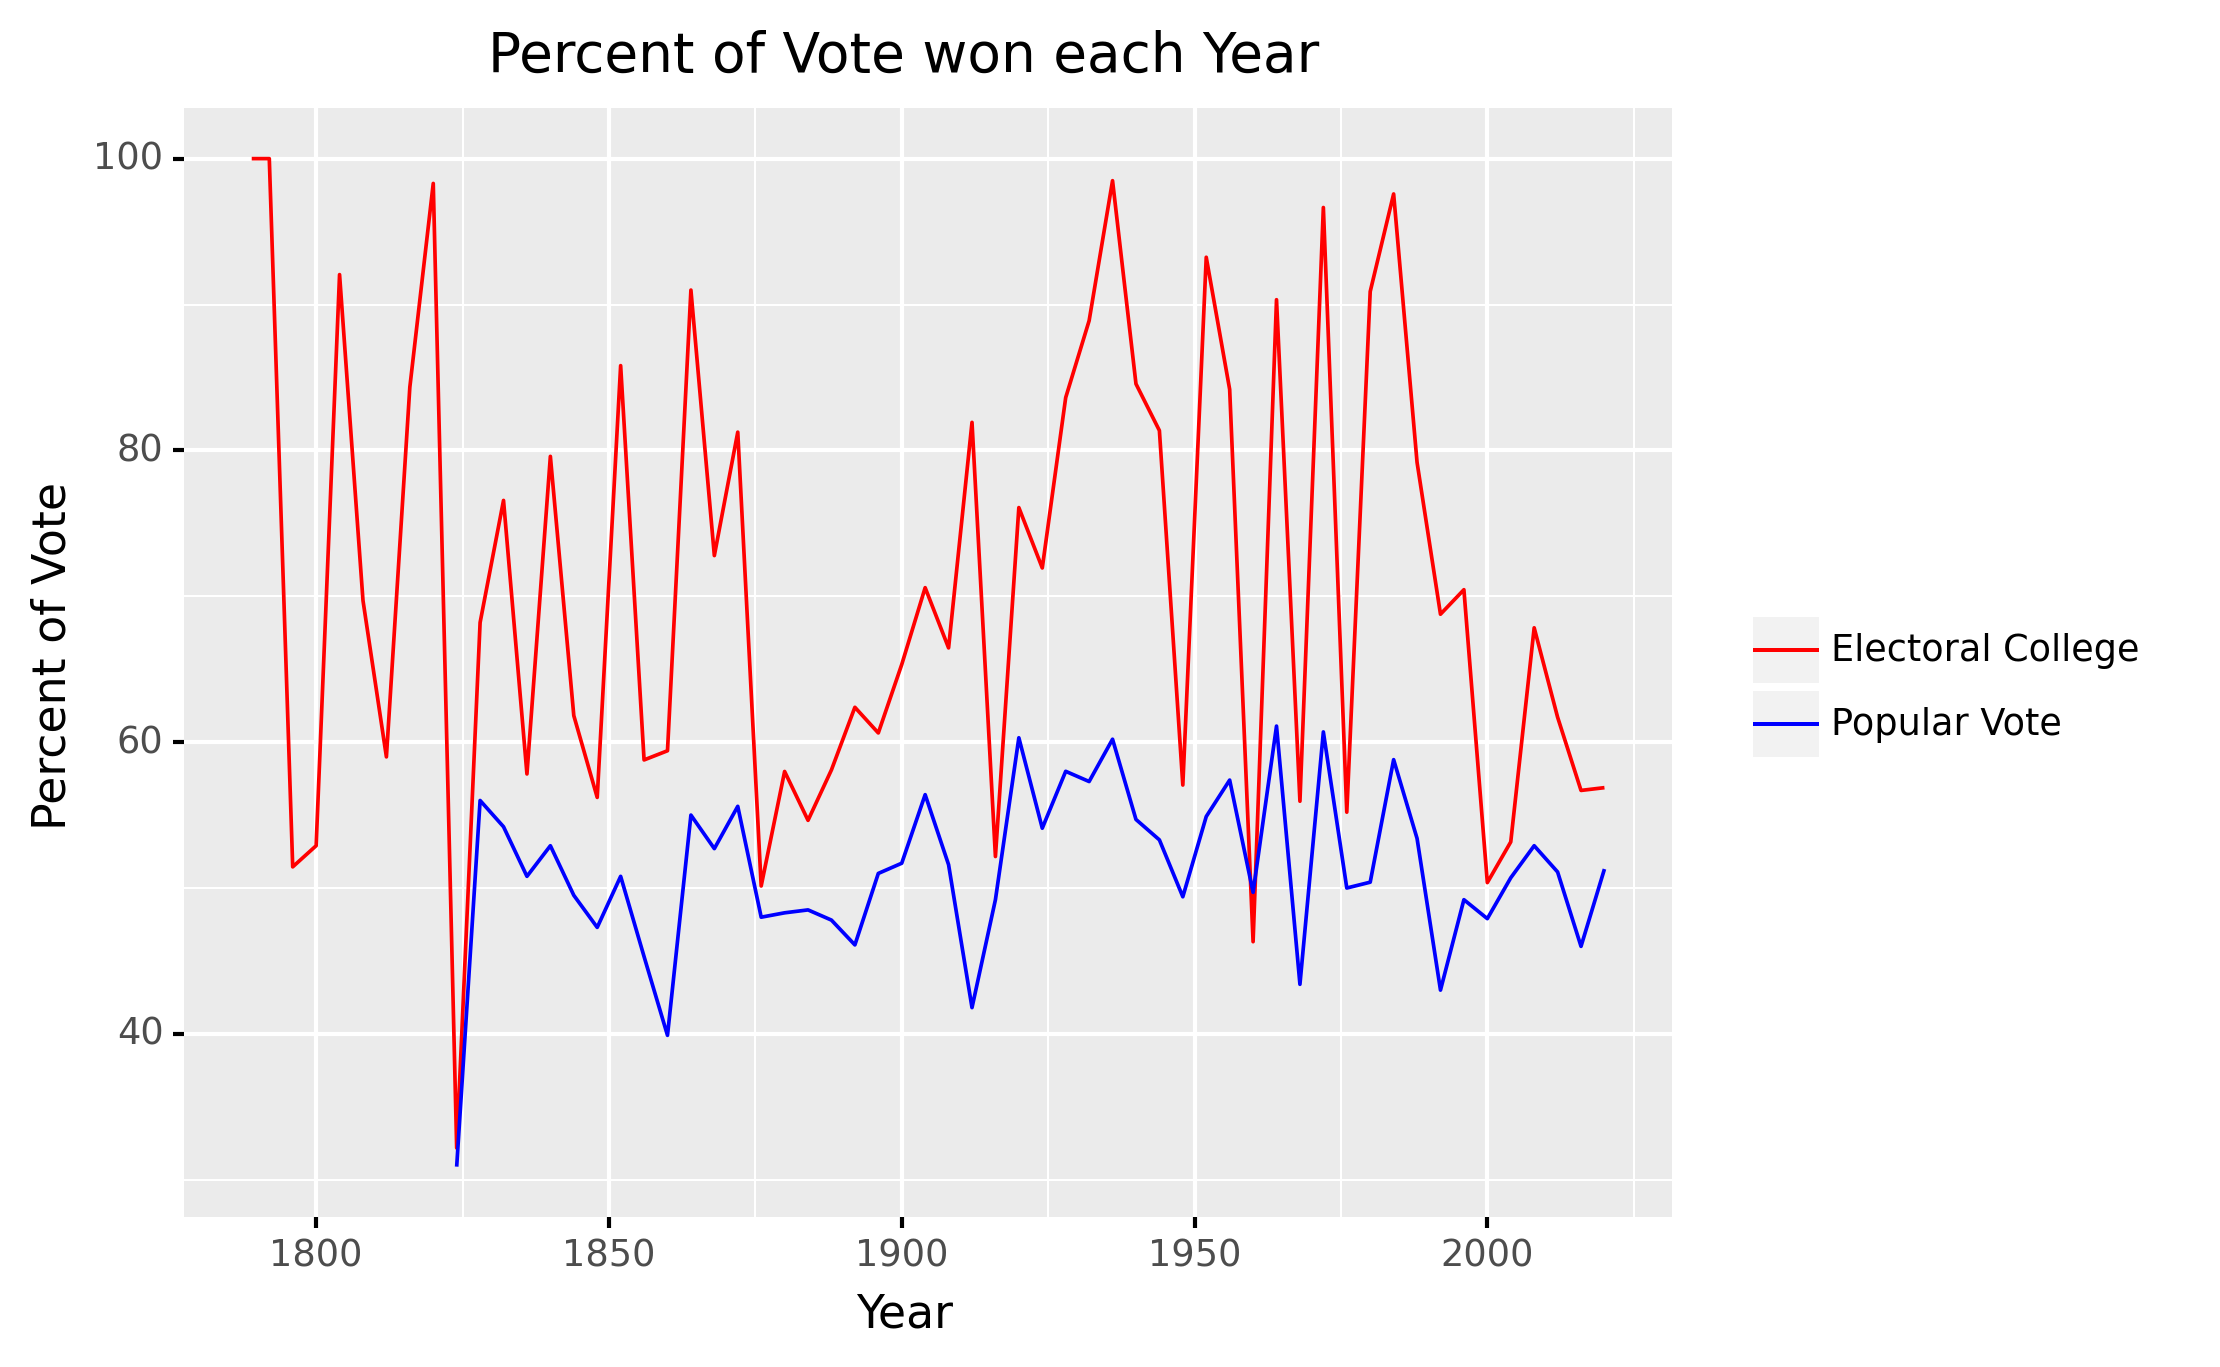
\includegraphics[width=0.9\linewidth]{election_results.png}
    \caption{Election Results}
\end{figure}

I also created a subset that only included the points where Change in GDP was measured - I knew that it would be a more limited dataset, but as economic growth has previously been a very significant measure of election results, I wanted to be able to look at it as well. 

\vspace{3.00mm}

Finally, I created two subsets where one included the swing states found from an overall historical view and the other with more current swing states, to be able to see which model was more accurate. I predicted that the overall swing state list would be more accurate, as it measures the cumulative accuracy, as opposed to the most recent accuracy. In Figure 3 below, it is not very intuitive which will be more accurate, so it will be useful to run my model with these two subsets independently to see my results. Both of these subsets treat Electoral College as the dependent variable and exclude GDP, a decision I made for simplicity and for focusing only on comparing these two subsets.

\begin{figure}[H]
    \begin{subfigure}
        \centering
        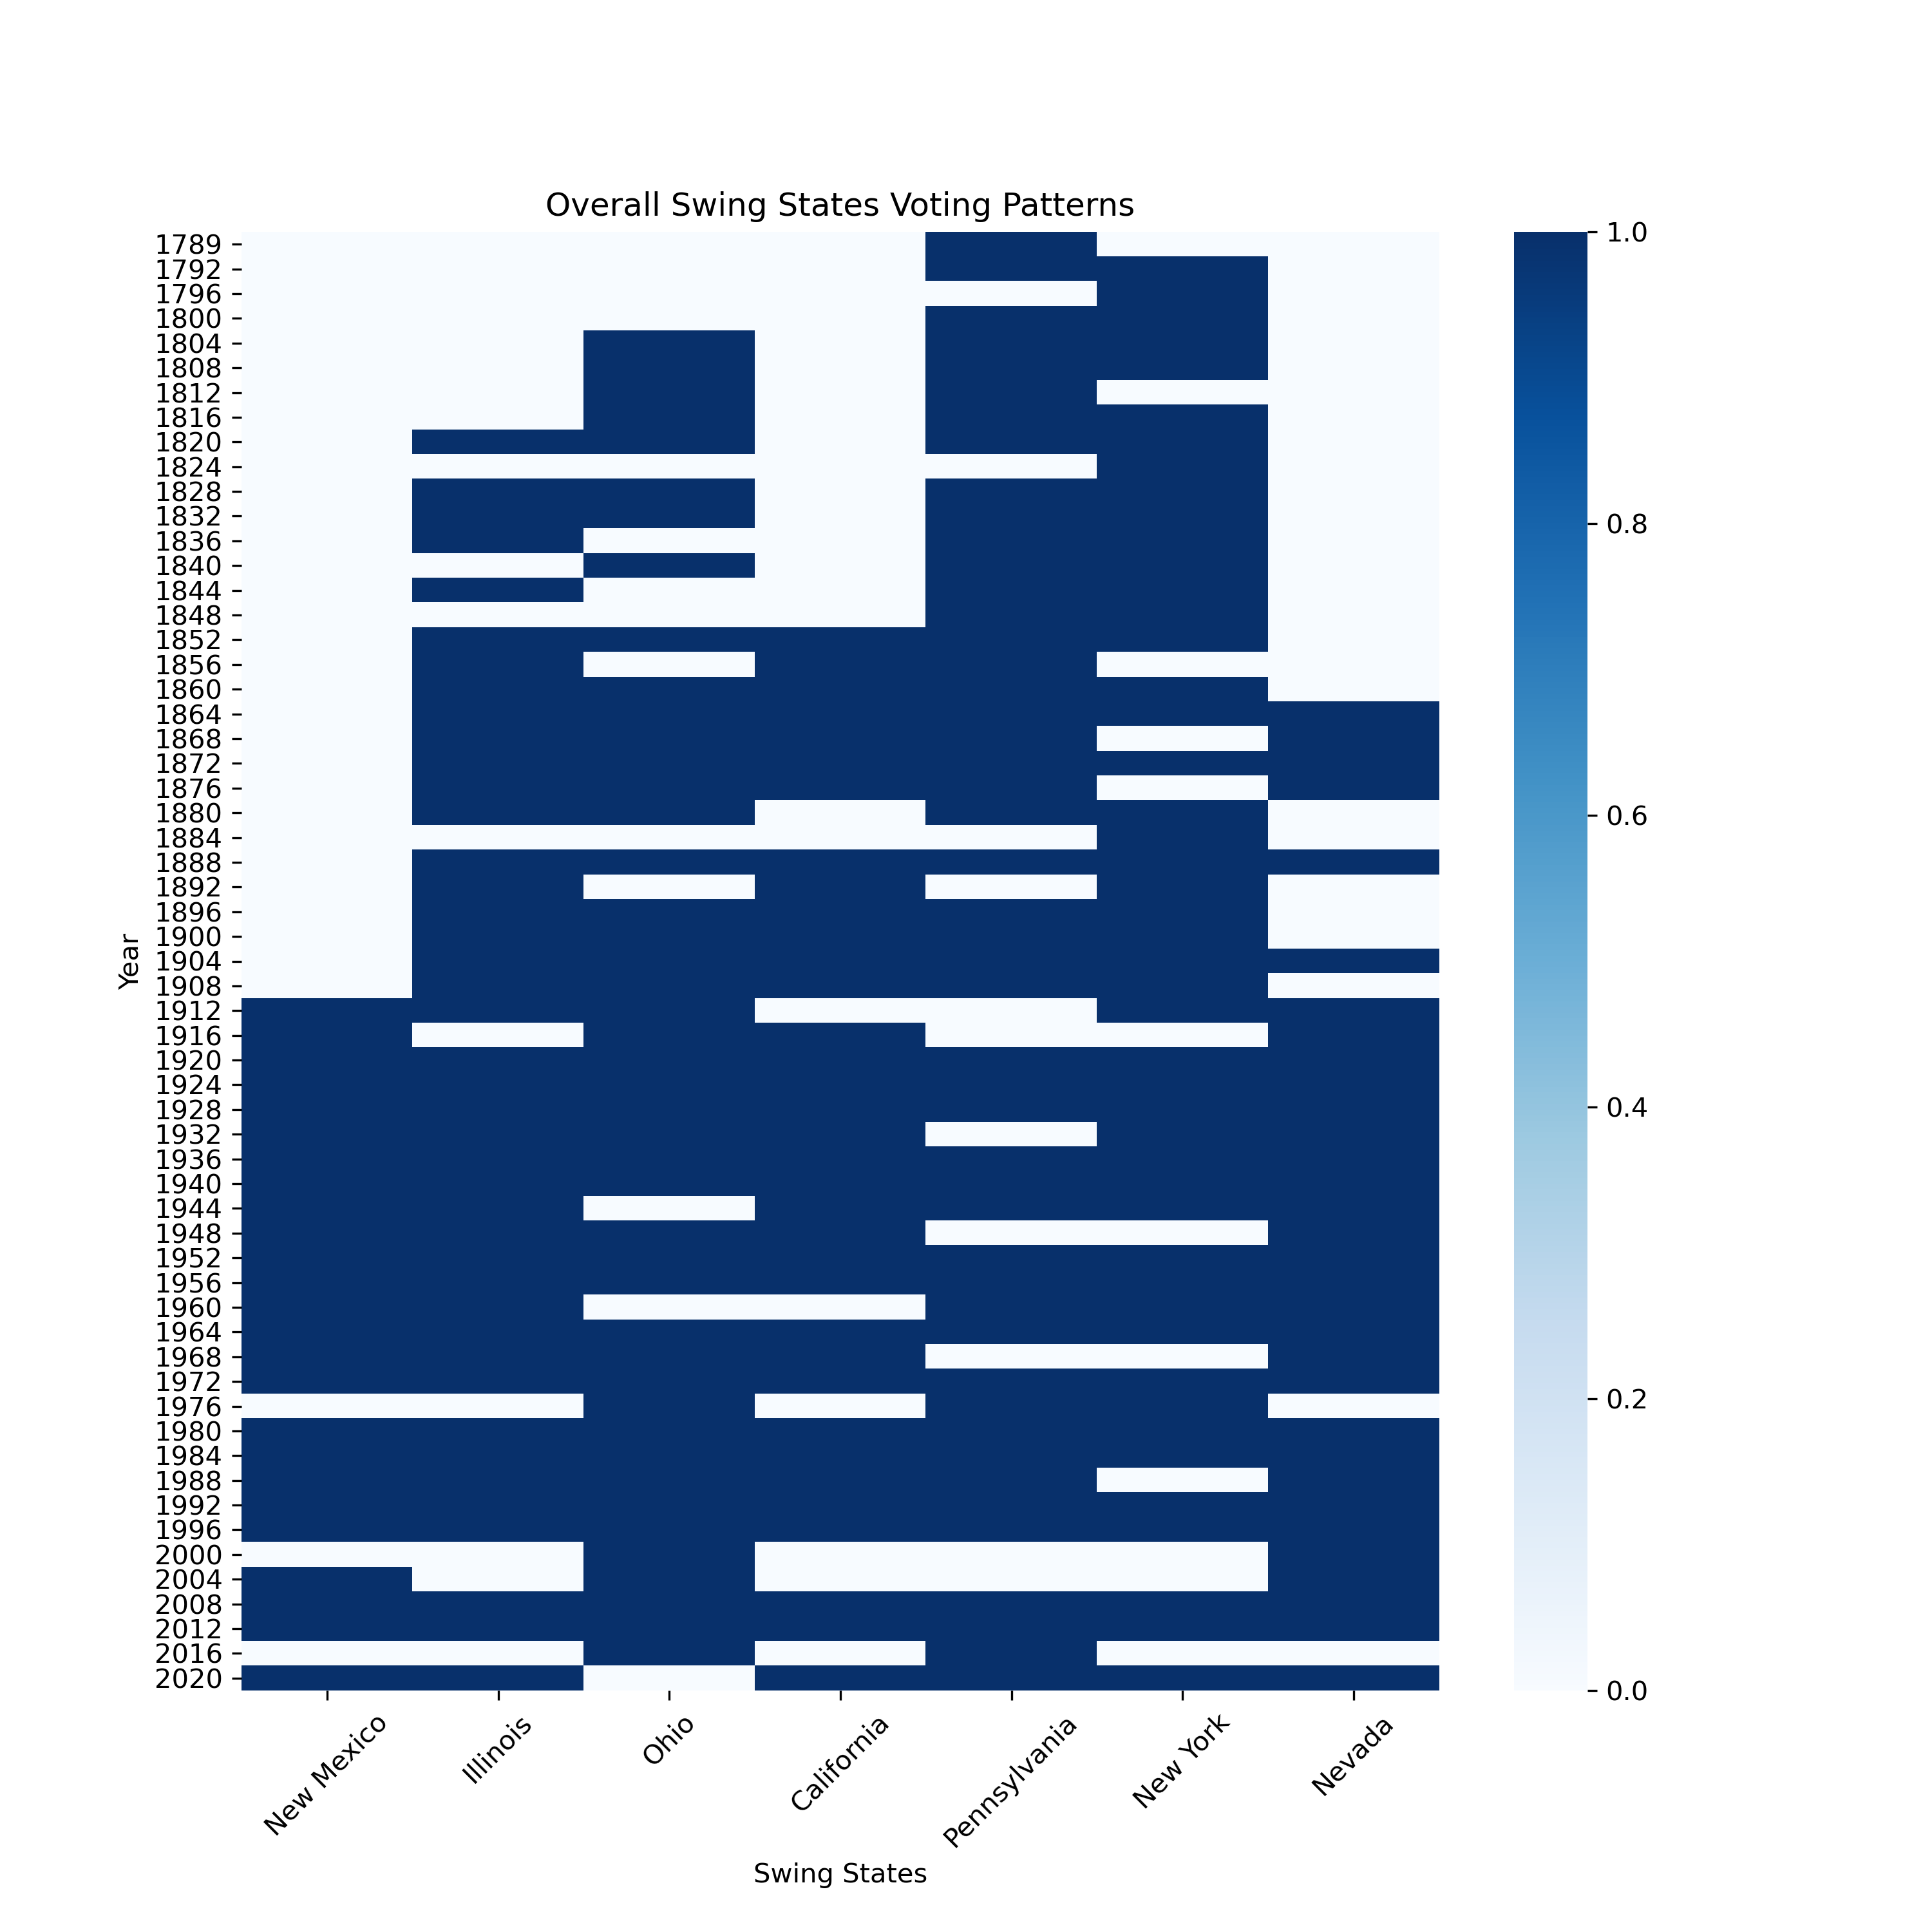
\includegraphics[width=0.6\linewidth]{Overall_Swing.png}
    \end{subfigure}
    \begin{subfigure}
        \centering
        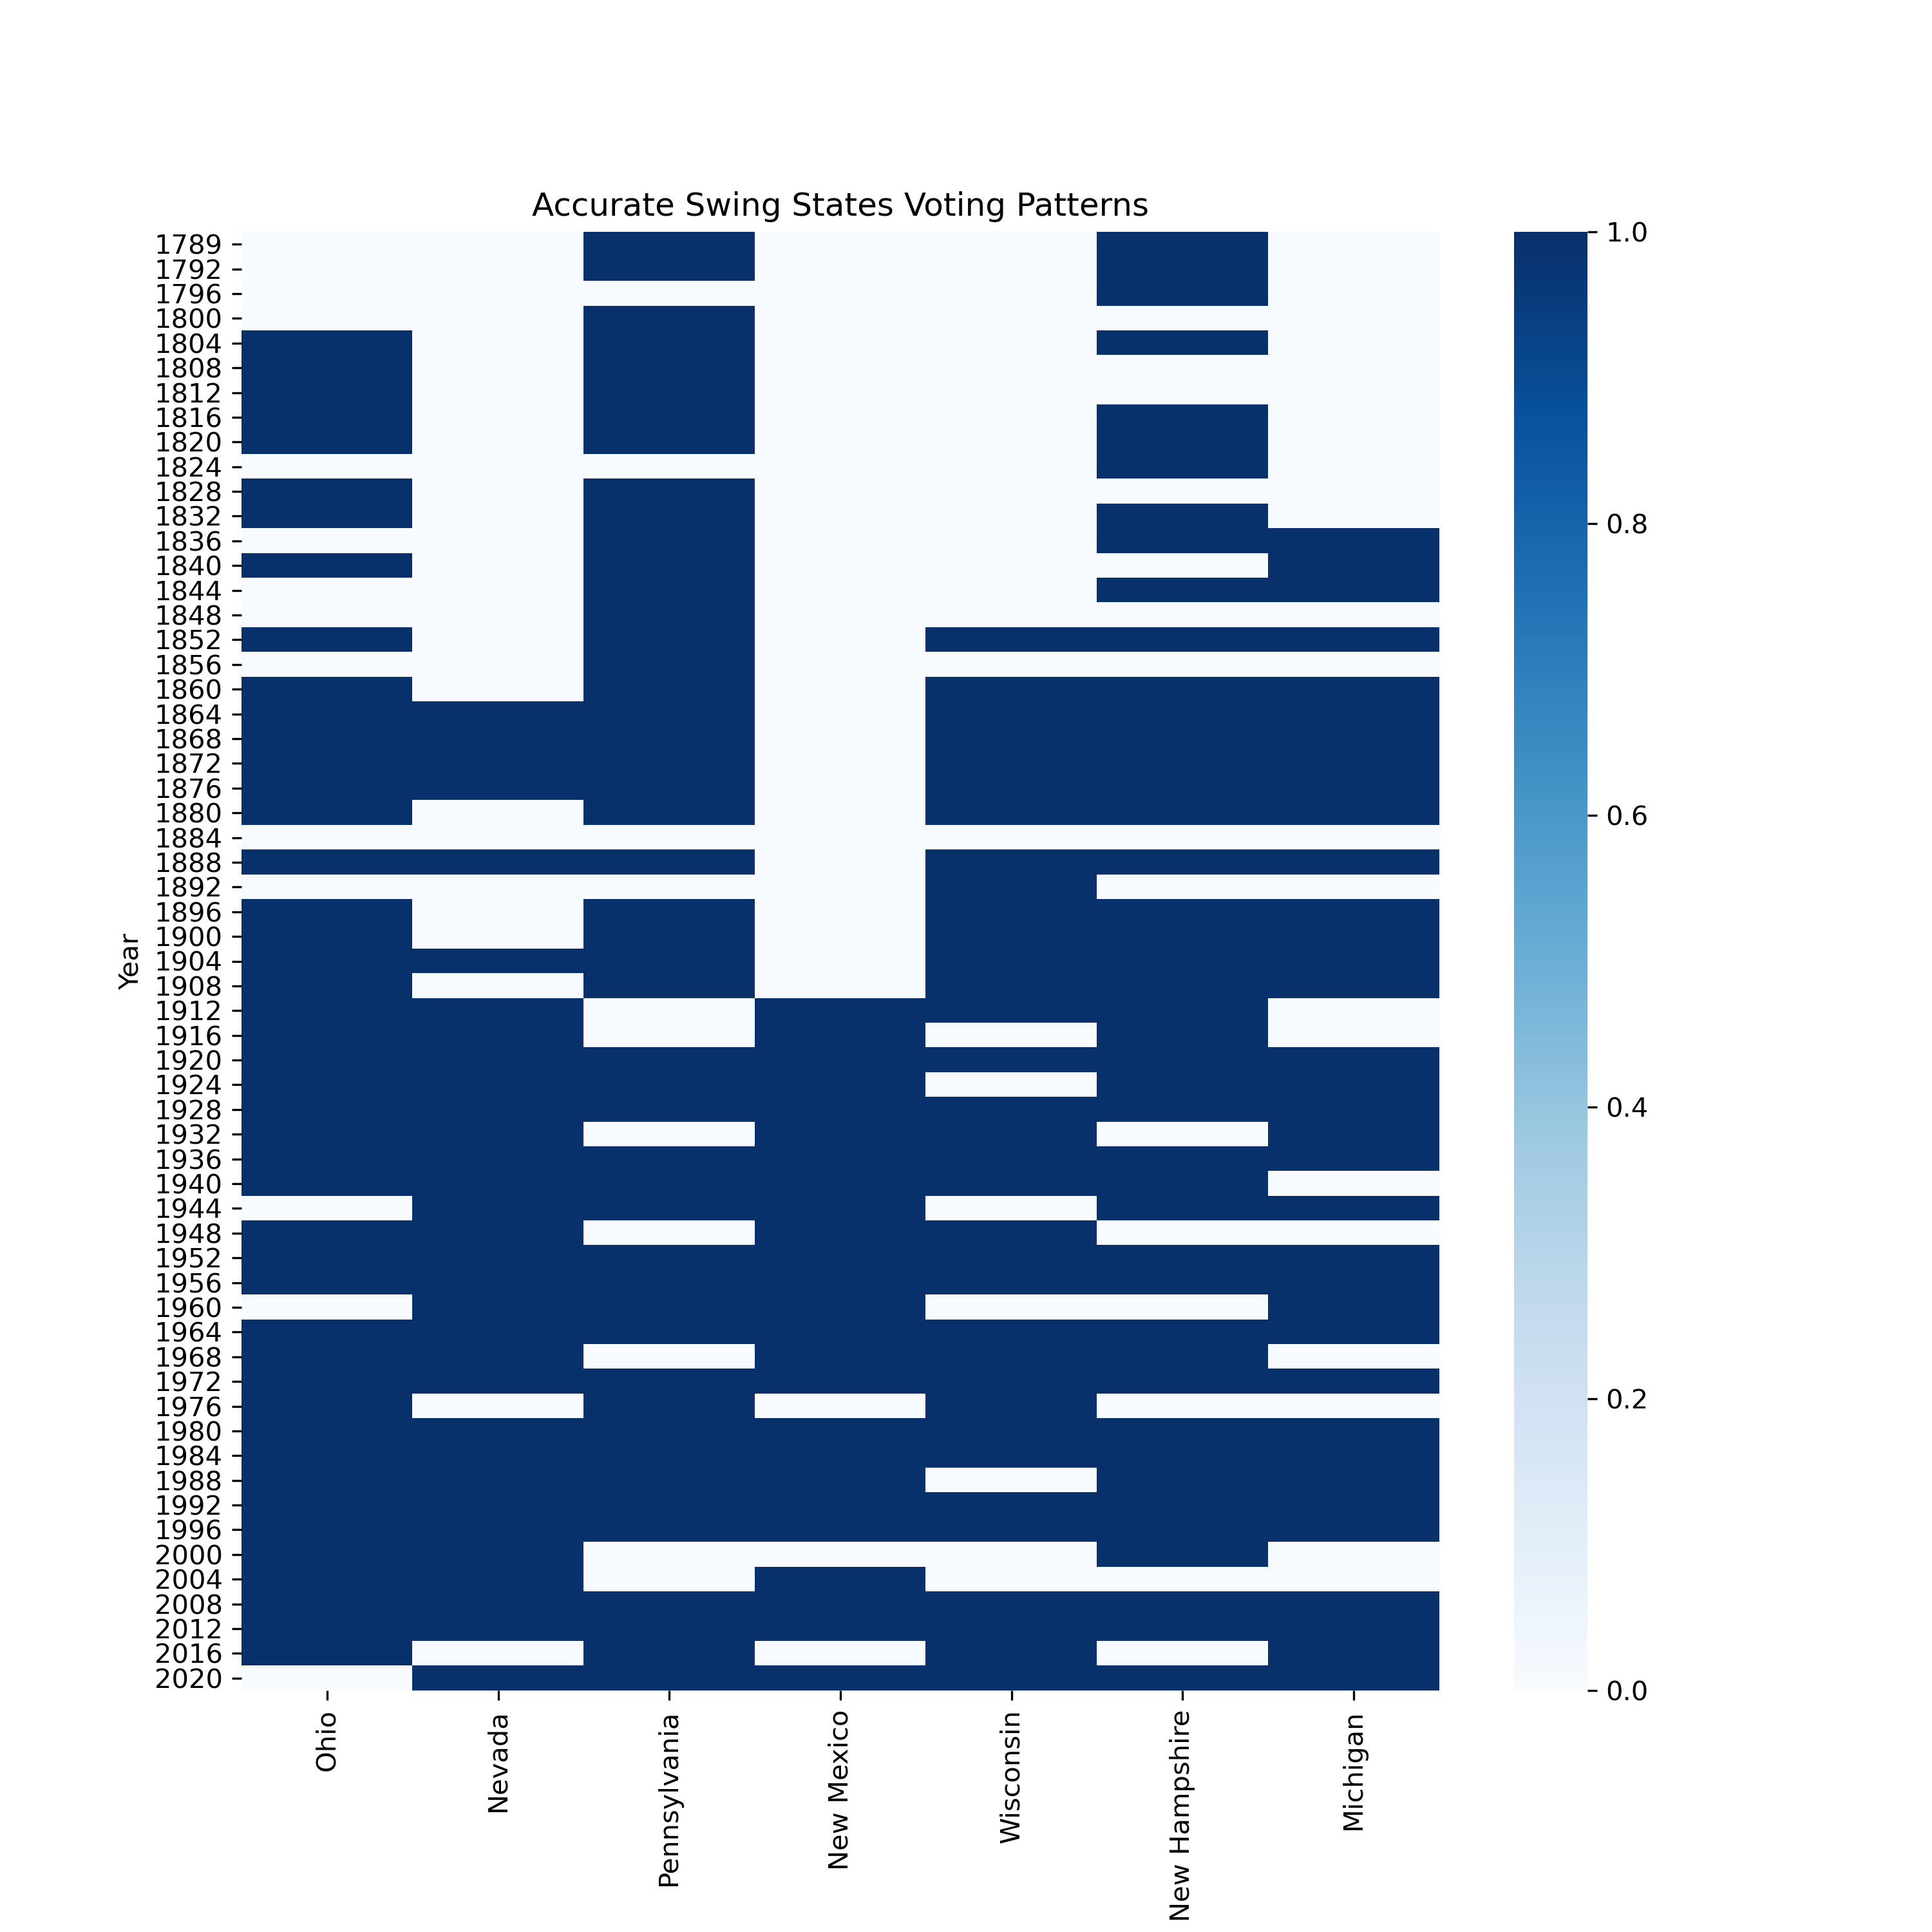
\includegraphics[width=0.6\linewidth]{Accurate_Swing.png}
    \end{subfigure}
    \caption{Overall and Accurate Swing State Heatmaps}
\end{figure}

I then took a look at some of the trends in the variables to get a sense of what my results might look like. The only real continuous independent variables were Change in GDP and Turnout Rate, so I looked to see whether there were any clear patterns there.

\begin{figure}[H]
    \centering
    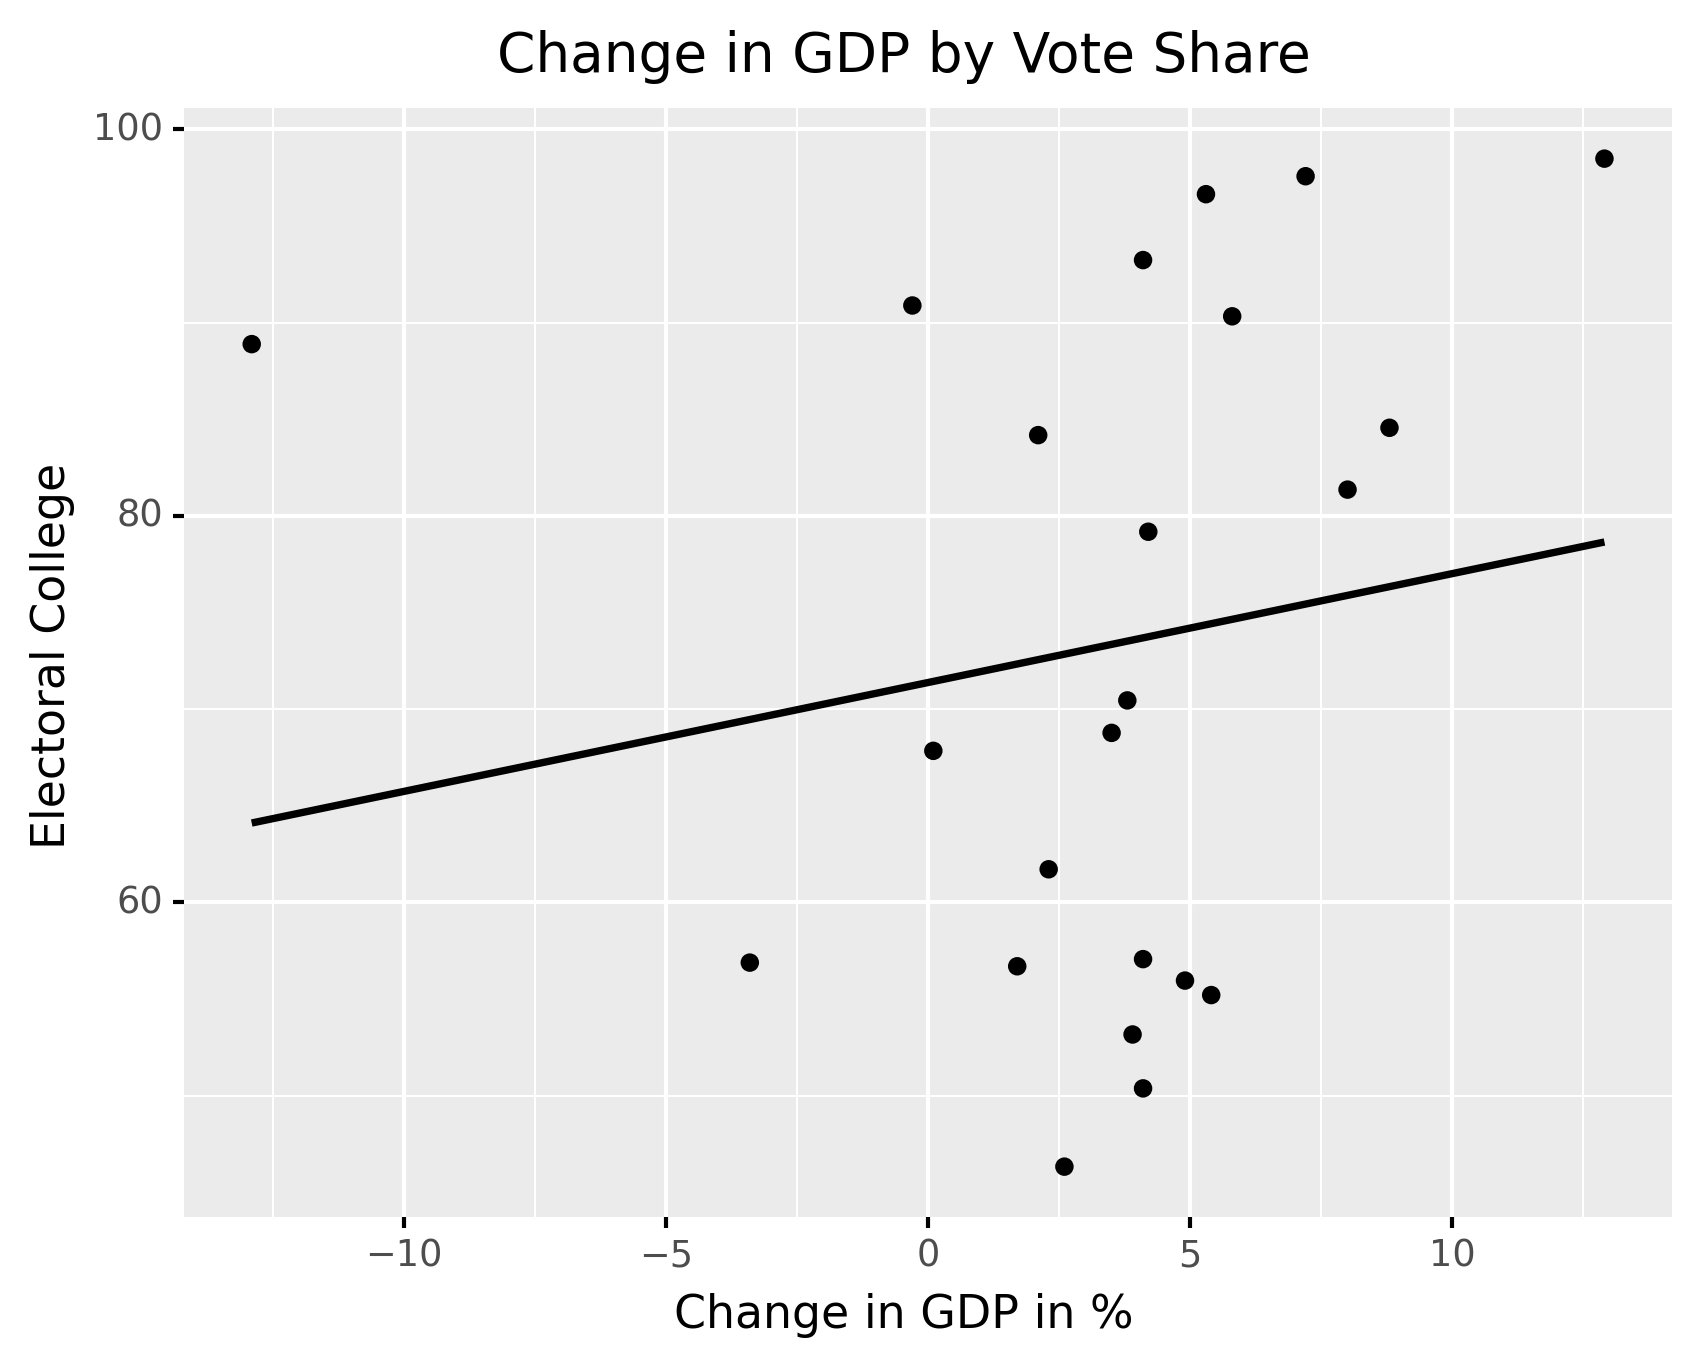
\includegraphics[width=0.6\linewidth]{gdp_by_share.png}
    \caption{Relationship between GDP and Vote Share}
\end{figure}

\vspace{3.00mm}

\begin{figure}[H]
    \centering
    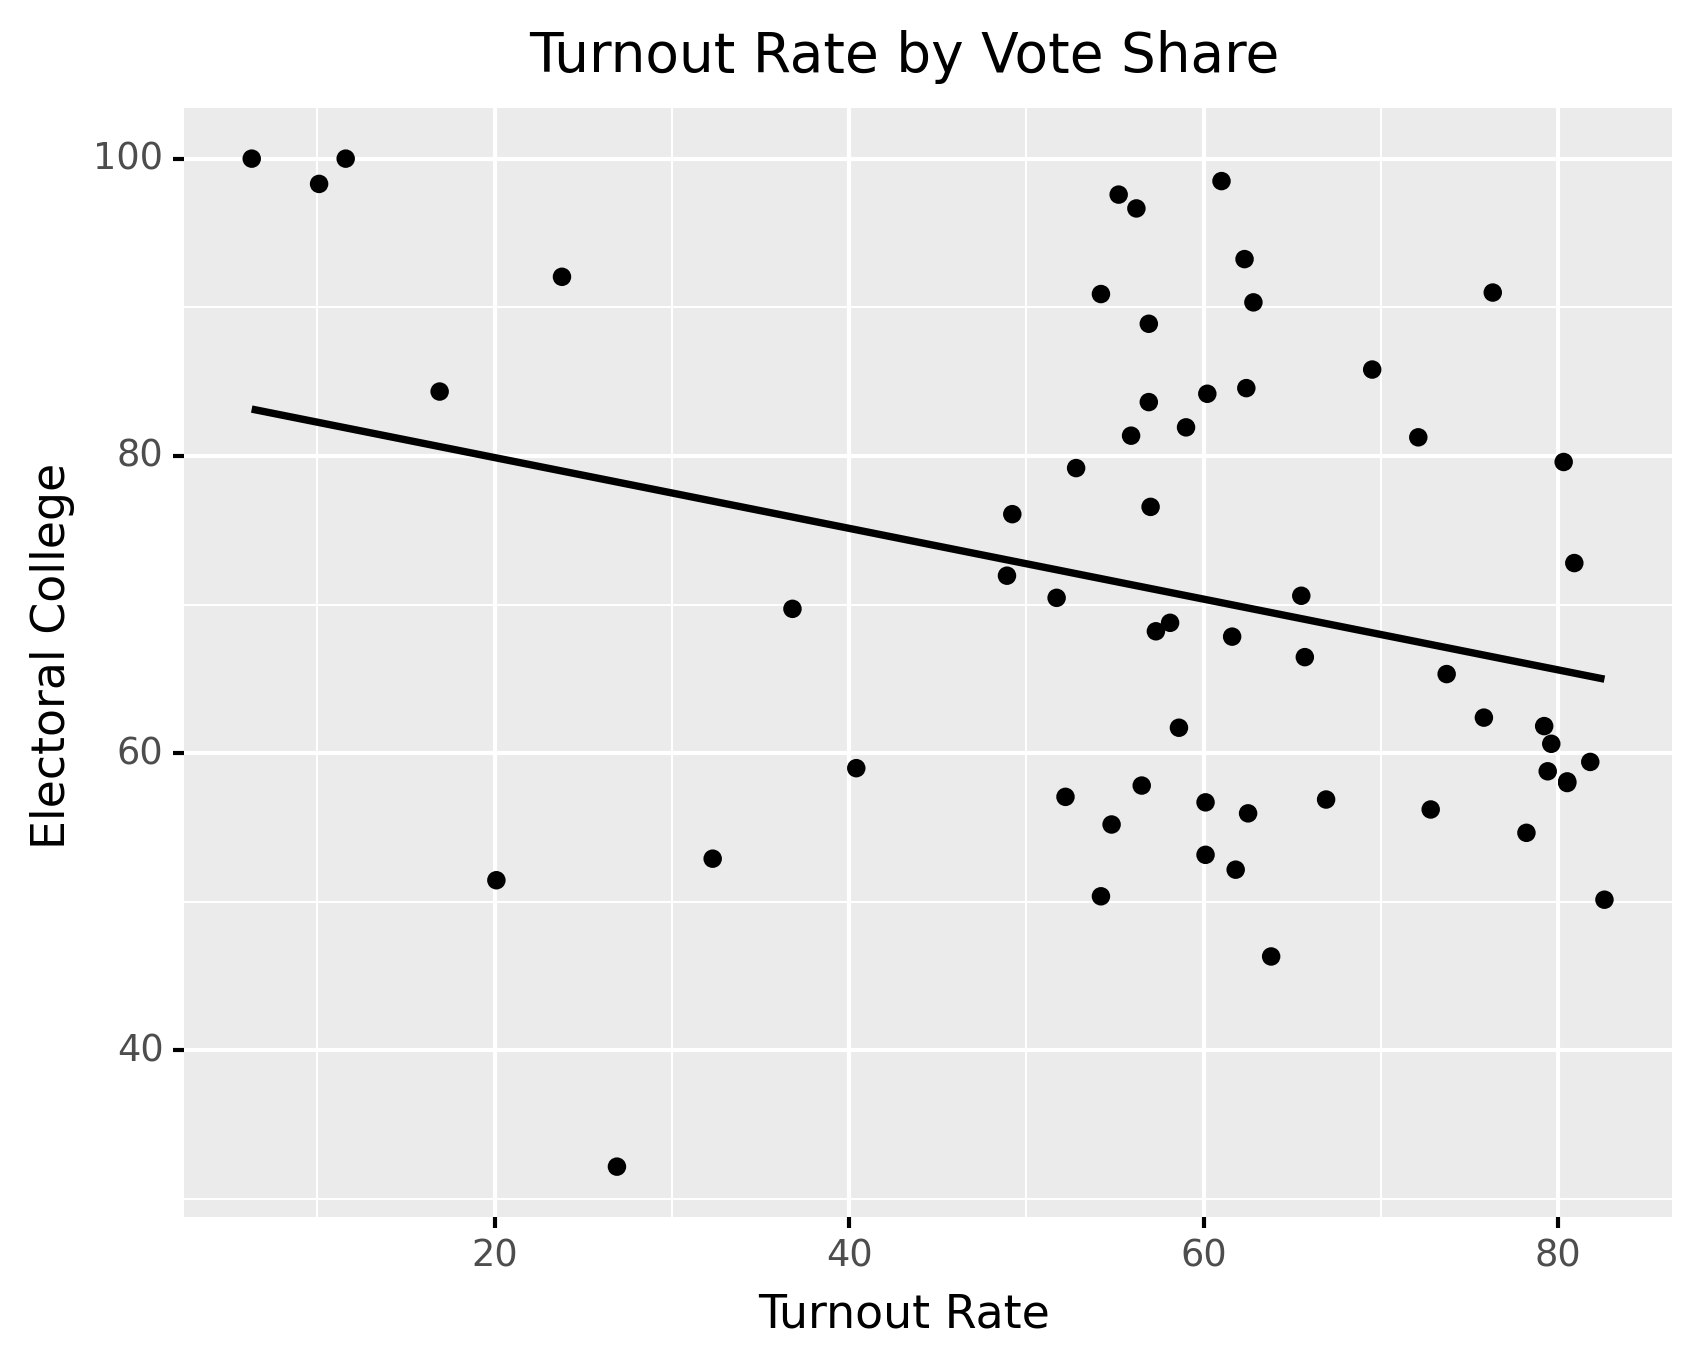
\includegraphics[width=0.6\linewidth]{turnout_by_share.png}
    \caption{Relationship between Turnout and Vote Share}
\end{figure}

It did look like there were some slight trends from these graphs, with Figure 4 having a positive correlation and Figure 5 having a negative correlation. I also took a look at some of the interactions with the dummy variables, such as how political party and incumbent status interact with the relationship between change in GDP and vote share as seen below in Figures 6 and 7.

\begin{figure}[H]
    \centering
    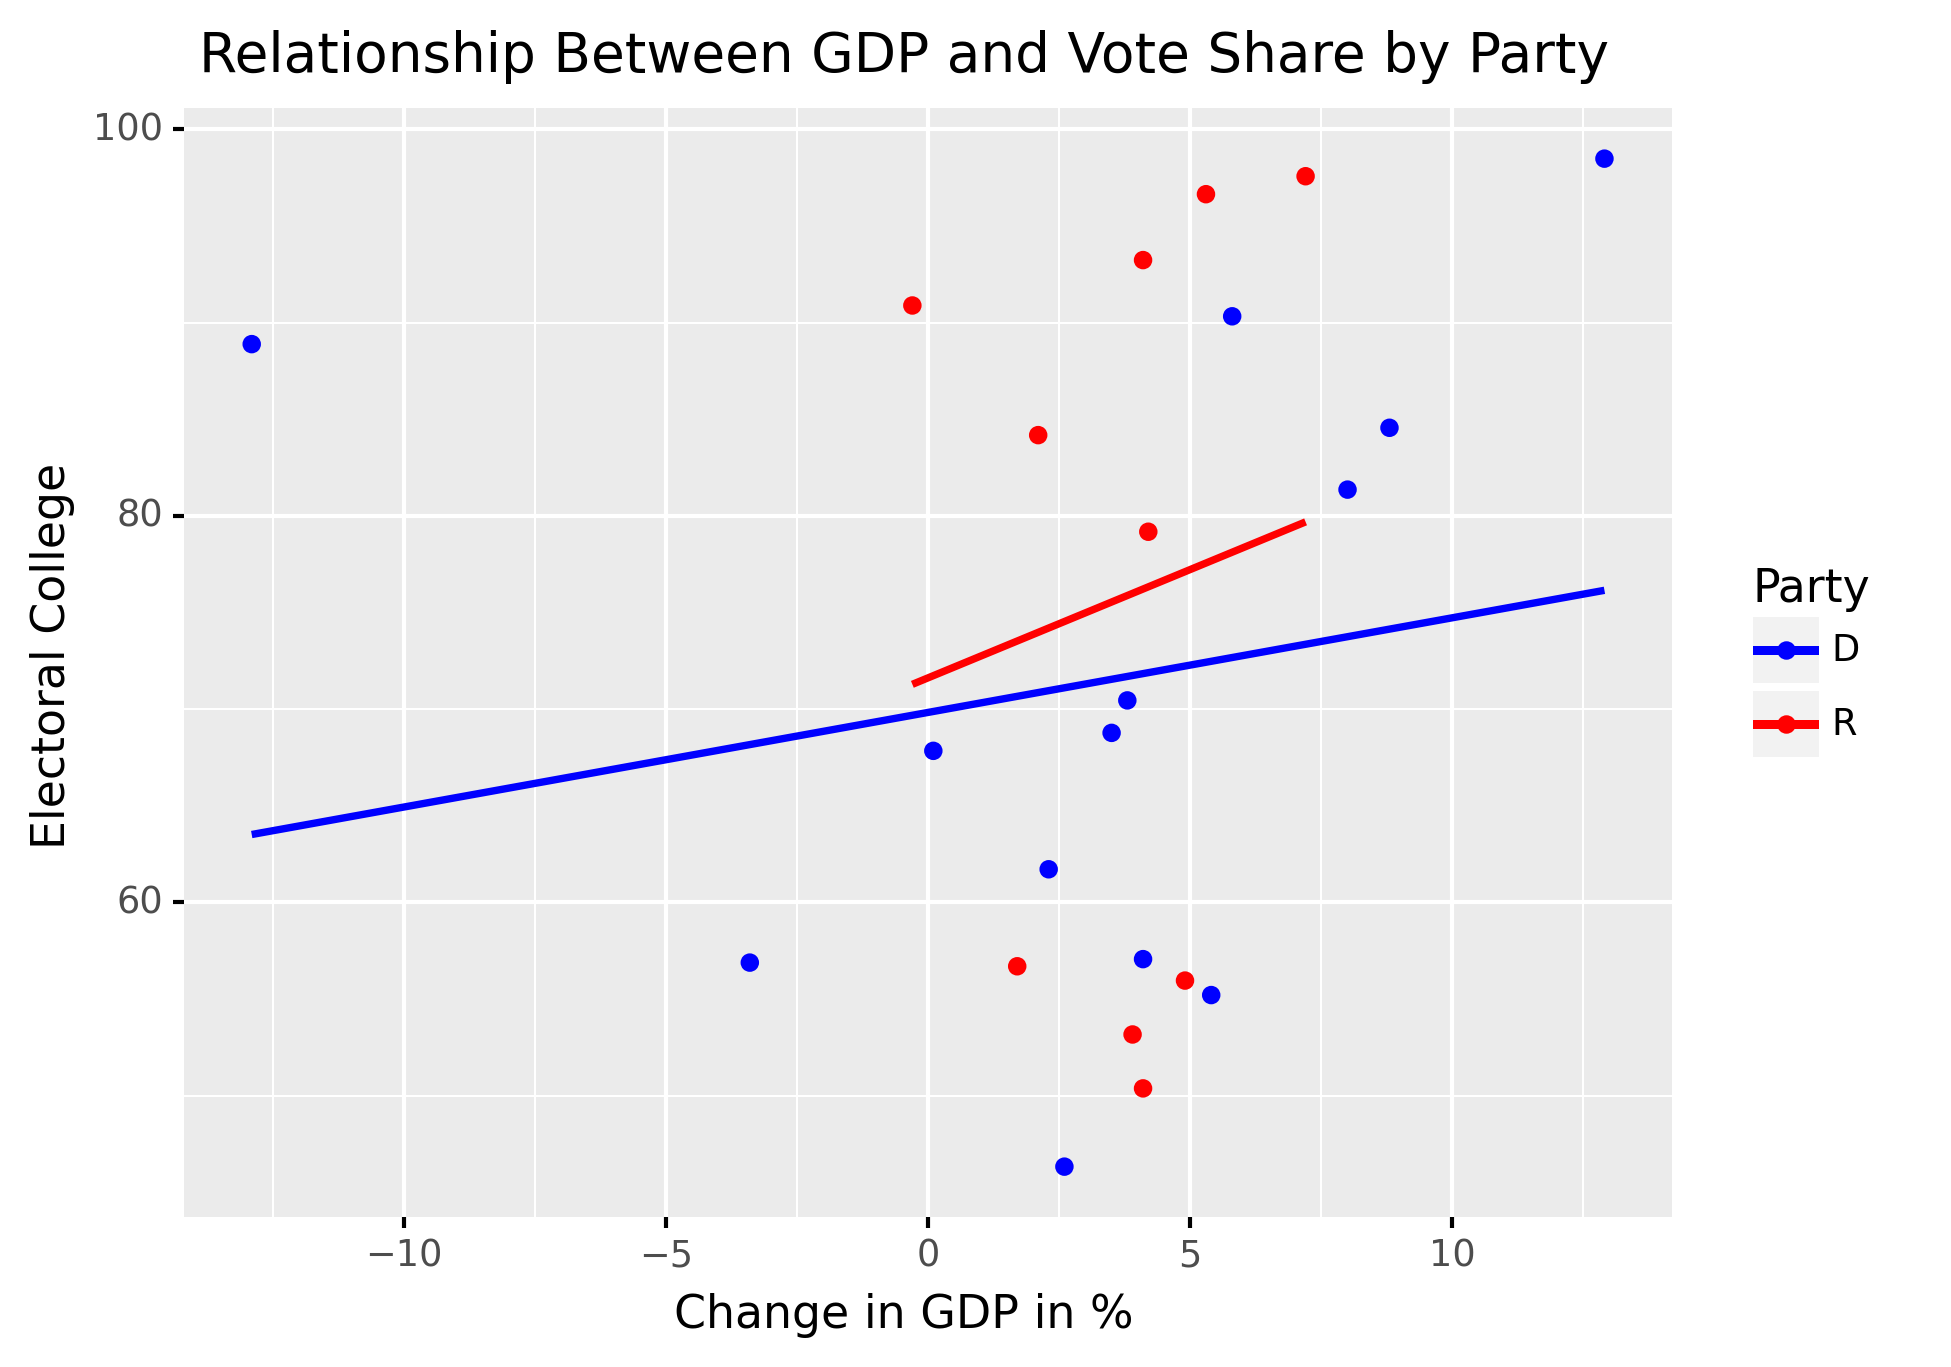
\includegraphics[width=0.6\linewidth]{gdp_party_share.png}
    \caption{Relationship between GDP and Vote Share by Party}
\end{figure}

\vspace{3.00mm}

\begin{figure}[H]
    \centering
    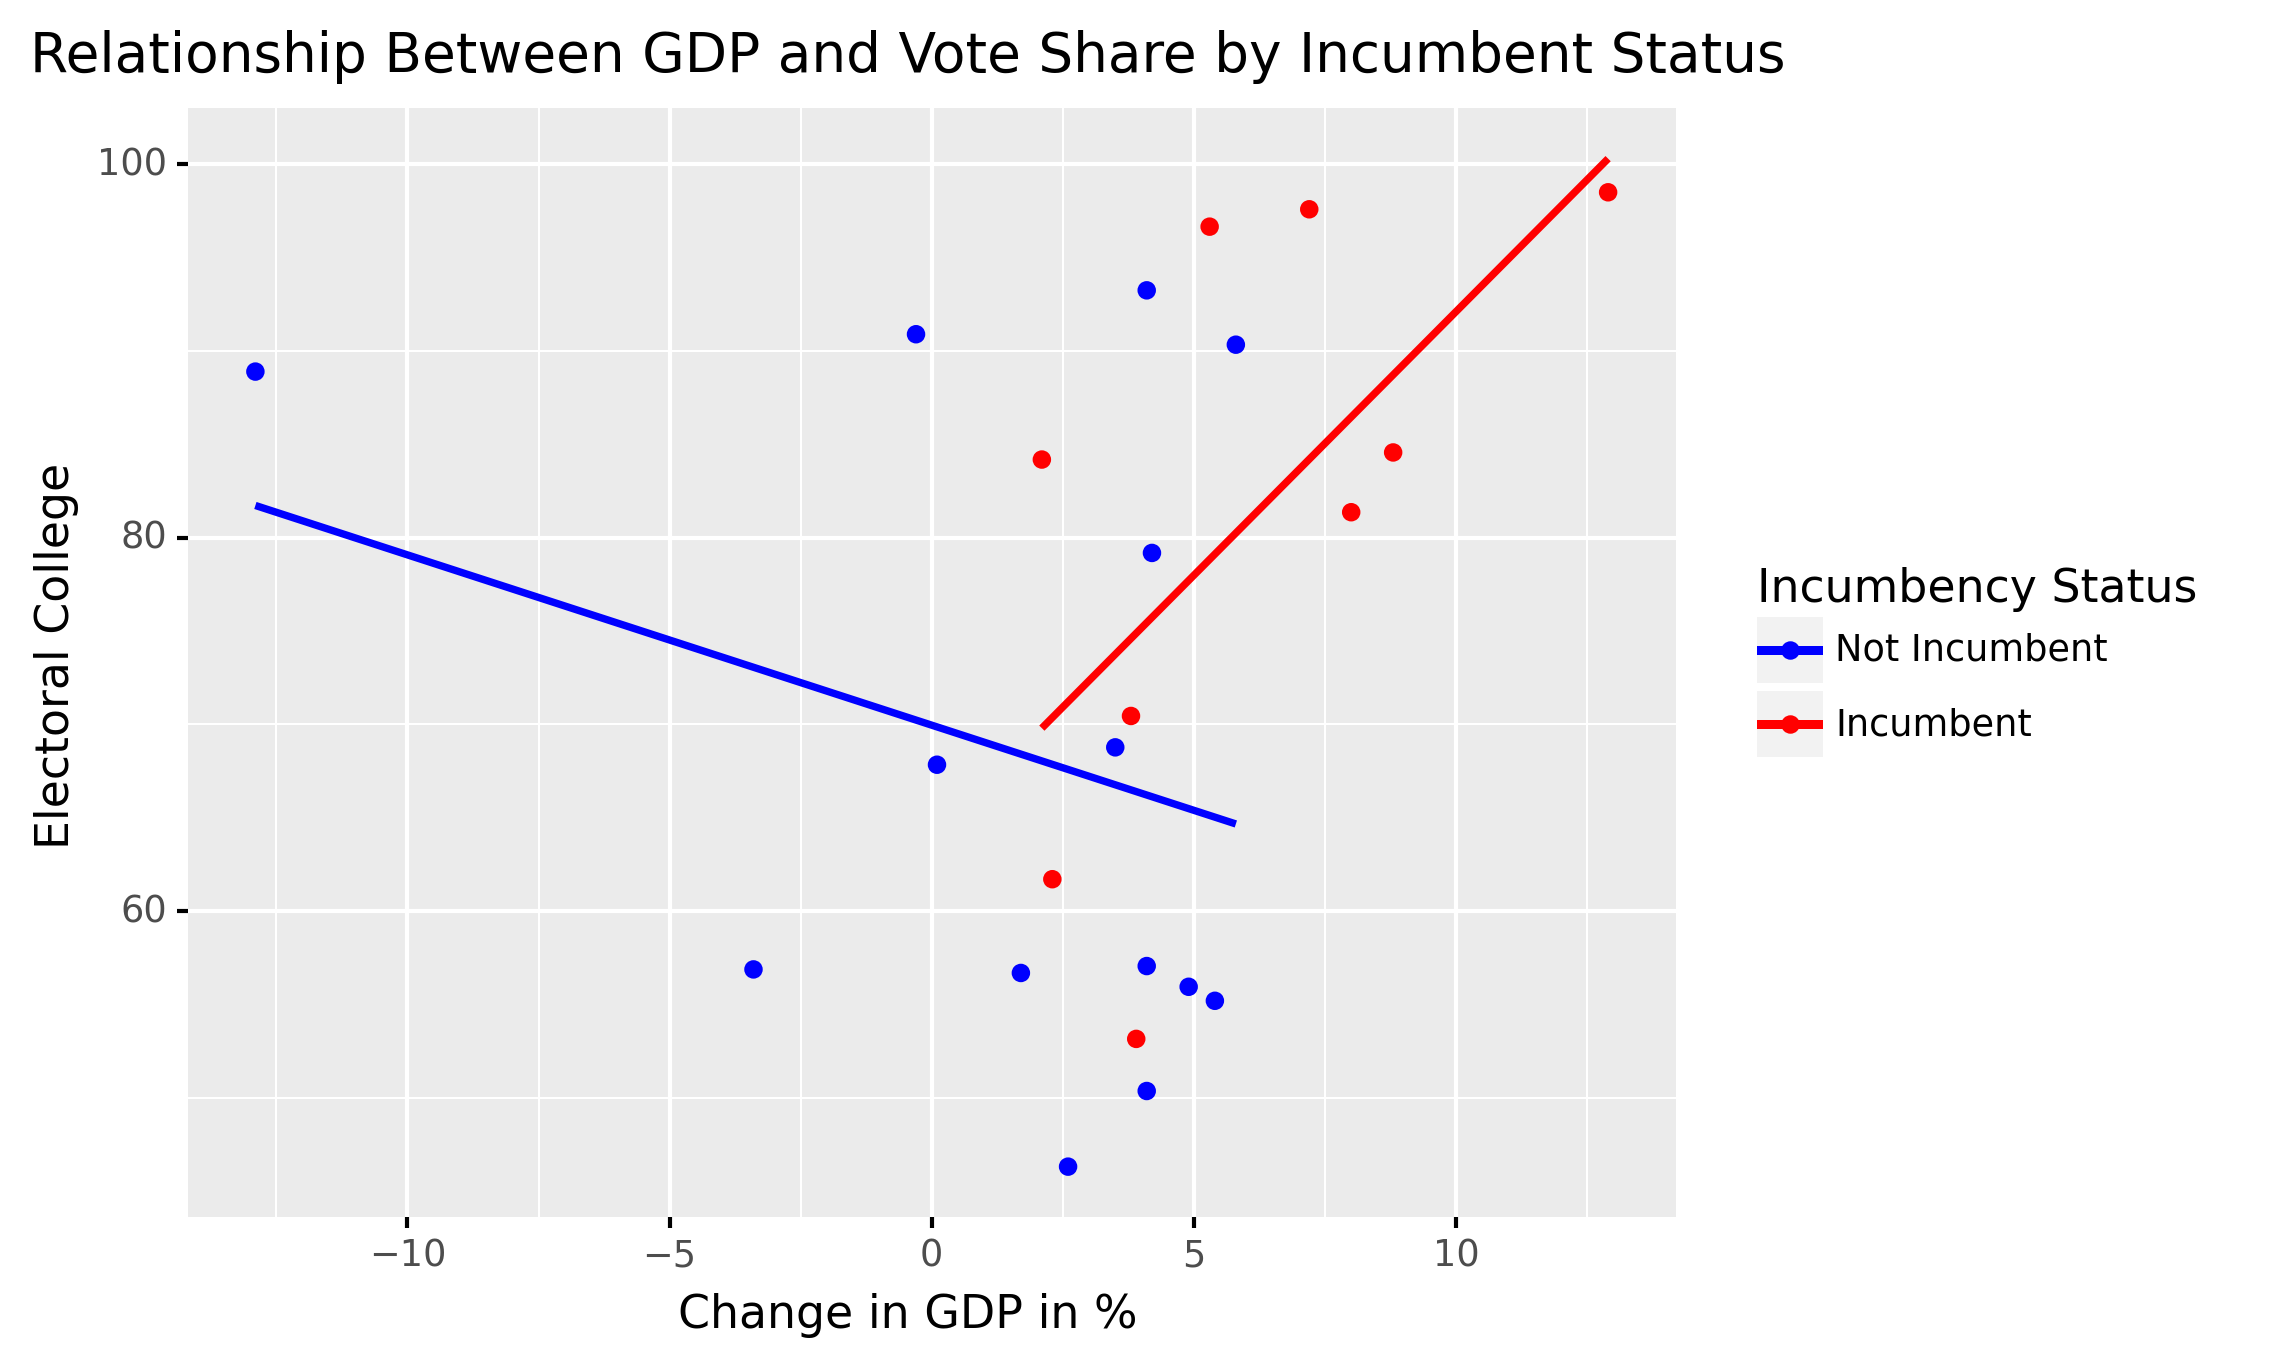
\includegraphics[width=0.7\linewidth]{gdp_incum_share.png}
    \caption{Relationship between GDP and Vote Share by Incumbent Status}
\end{figure}

There were some clear and interesting trends here, and you can see how including interaction variables in the model would likely give some more accurate results. In further analyses of this project, I would add in actual interaction variables into my dataset and see how it affects the model.

\vspace{3.00mm}

For the modeling section of my analysis, as my dependent variables were continuous, I had to choose models that weren't solely focused on classification. Therefore, I included a Linear Model, a Bagging Model, K-Nearest Neighbors, Decision Trees, and Random Forests in my search space. The scoring parameter I decided to use is \verb|neg_mean_squared_error| because it is relatively simple to interpret - the lower the score, the better the fit, and the square root of this number will approximately represent the average distance between the predicted values and the actual values of the dependent variable. Because of my low sample size, I split my data into training and testing data with 80\% of the data going into the training set and only 20\% in the testing set. Then, in determining variable importance, I used \verb|permutation_importance| and partial dependency plots to visualize how to features differed. 

\section*{Results}

When I ran each of my models using the different subsets I created, I found that there were pretty different levels of accuracy depending on the subset. A summary of my results can be seen from Figure 8 below, which I exported using \verb|dataframe_image|.

\begin{figure}[H]
    \centering
    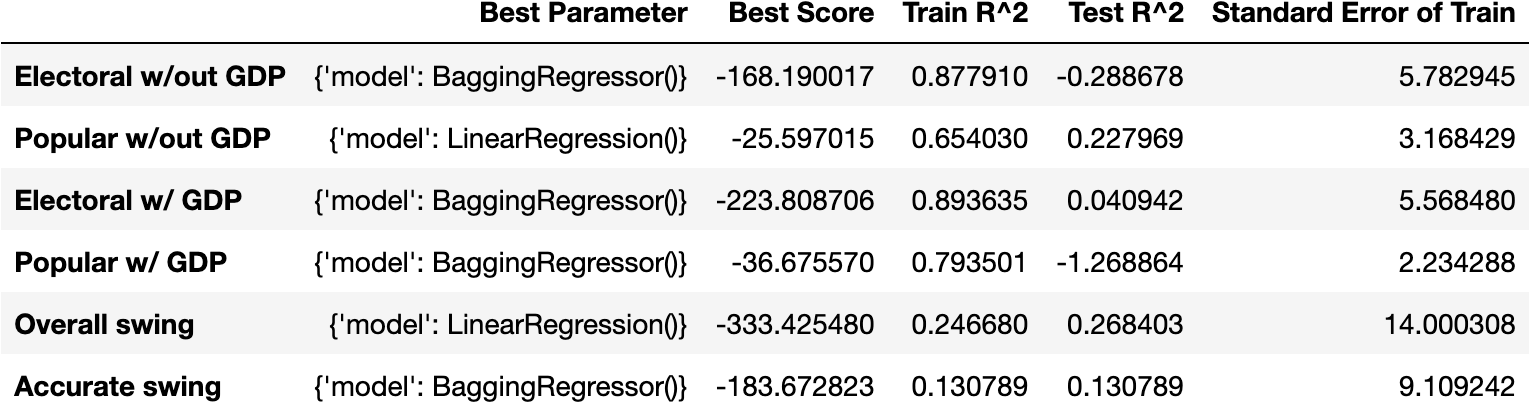
\includegraphics[width=0.9\linewidth]{Comparing_Results.png}
    \caption{Results from Models from Different Subsets}
\end{figure}

For most of the subsets, the Bagging Regressor ended up being the best parameter, though it did vary each time the models were ran. The best scores for the Bagging Regressor and the Linear Regression were likely very similar. One notable result is that the subsets that used the Popular Vote as the dependent variable had significantly lower scores. However, this is potentially because the actual values for the Popular Vote were mostly lower than the values for Electoral College. When comparing the standard error of the training data, which was calculated by taking the square root of the mean squared error, the results from the Popular Vote sets were still lower, but more similar. With this data, the vote share represents a percent, so we can interpret the standard error is being number of percentage points difference between the predicted values and actual values. 

\vspace{3.00mm}

There are some different ways of assessing which subset ran the best model. The subset using Popular Vote as the dependent variable without GDP included has the lowest best score, and the subset using Popular Vote with GDP included has the lowest standard error. However, as mentioned previously, this doesn't necessarily mean that they were better models. A better way of determining this is the R-squared values. The R-squared for the training data is highest in the subset that uses Electoral College as the dependent variable and includes GDP. This value indicates that 89\% of the model fits the observed data, which seems pretty good. The R-squared values for the test data is much worse for all of the subsets, with even a couple negative values. Looking at the test R-squared for the first four subsets, the subset that uses Popular Vote without GDP is the highest.

\vspace{3.00mm}

The results for the swing states was also mixed - The R-squared values were higher for the overall swing states, but the score and standard error were lower for the current more accurate swing states. If we view R-squared as the most important factor in assessing significance, then I was correct and the overall swing states are more predictive than the currently accurate swing states.

\vspace{3.00mm}

I decided to use the subset that uses Electoral College as the dependent variable and includes GDP to look at the relative importance of the variables, as it had the highest R-squared. After permuting the features 25 times, we can see from Figure 9 below that the most significant non-state feature is Change in GDP, which was expected. California is somewhat surprisingly the most important feature, but most of the other states are lower down in importance.

\begin{figure}[H]
    \centering
    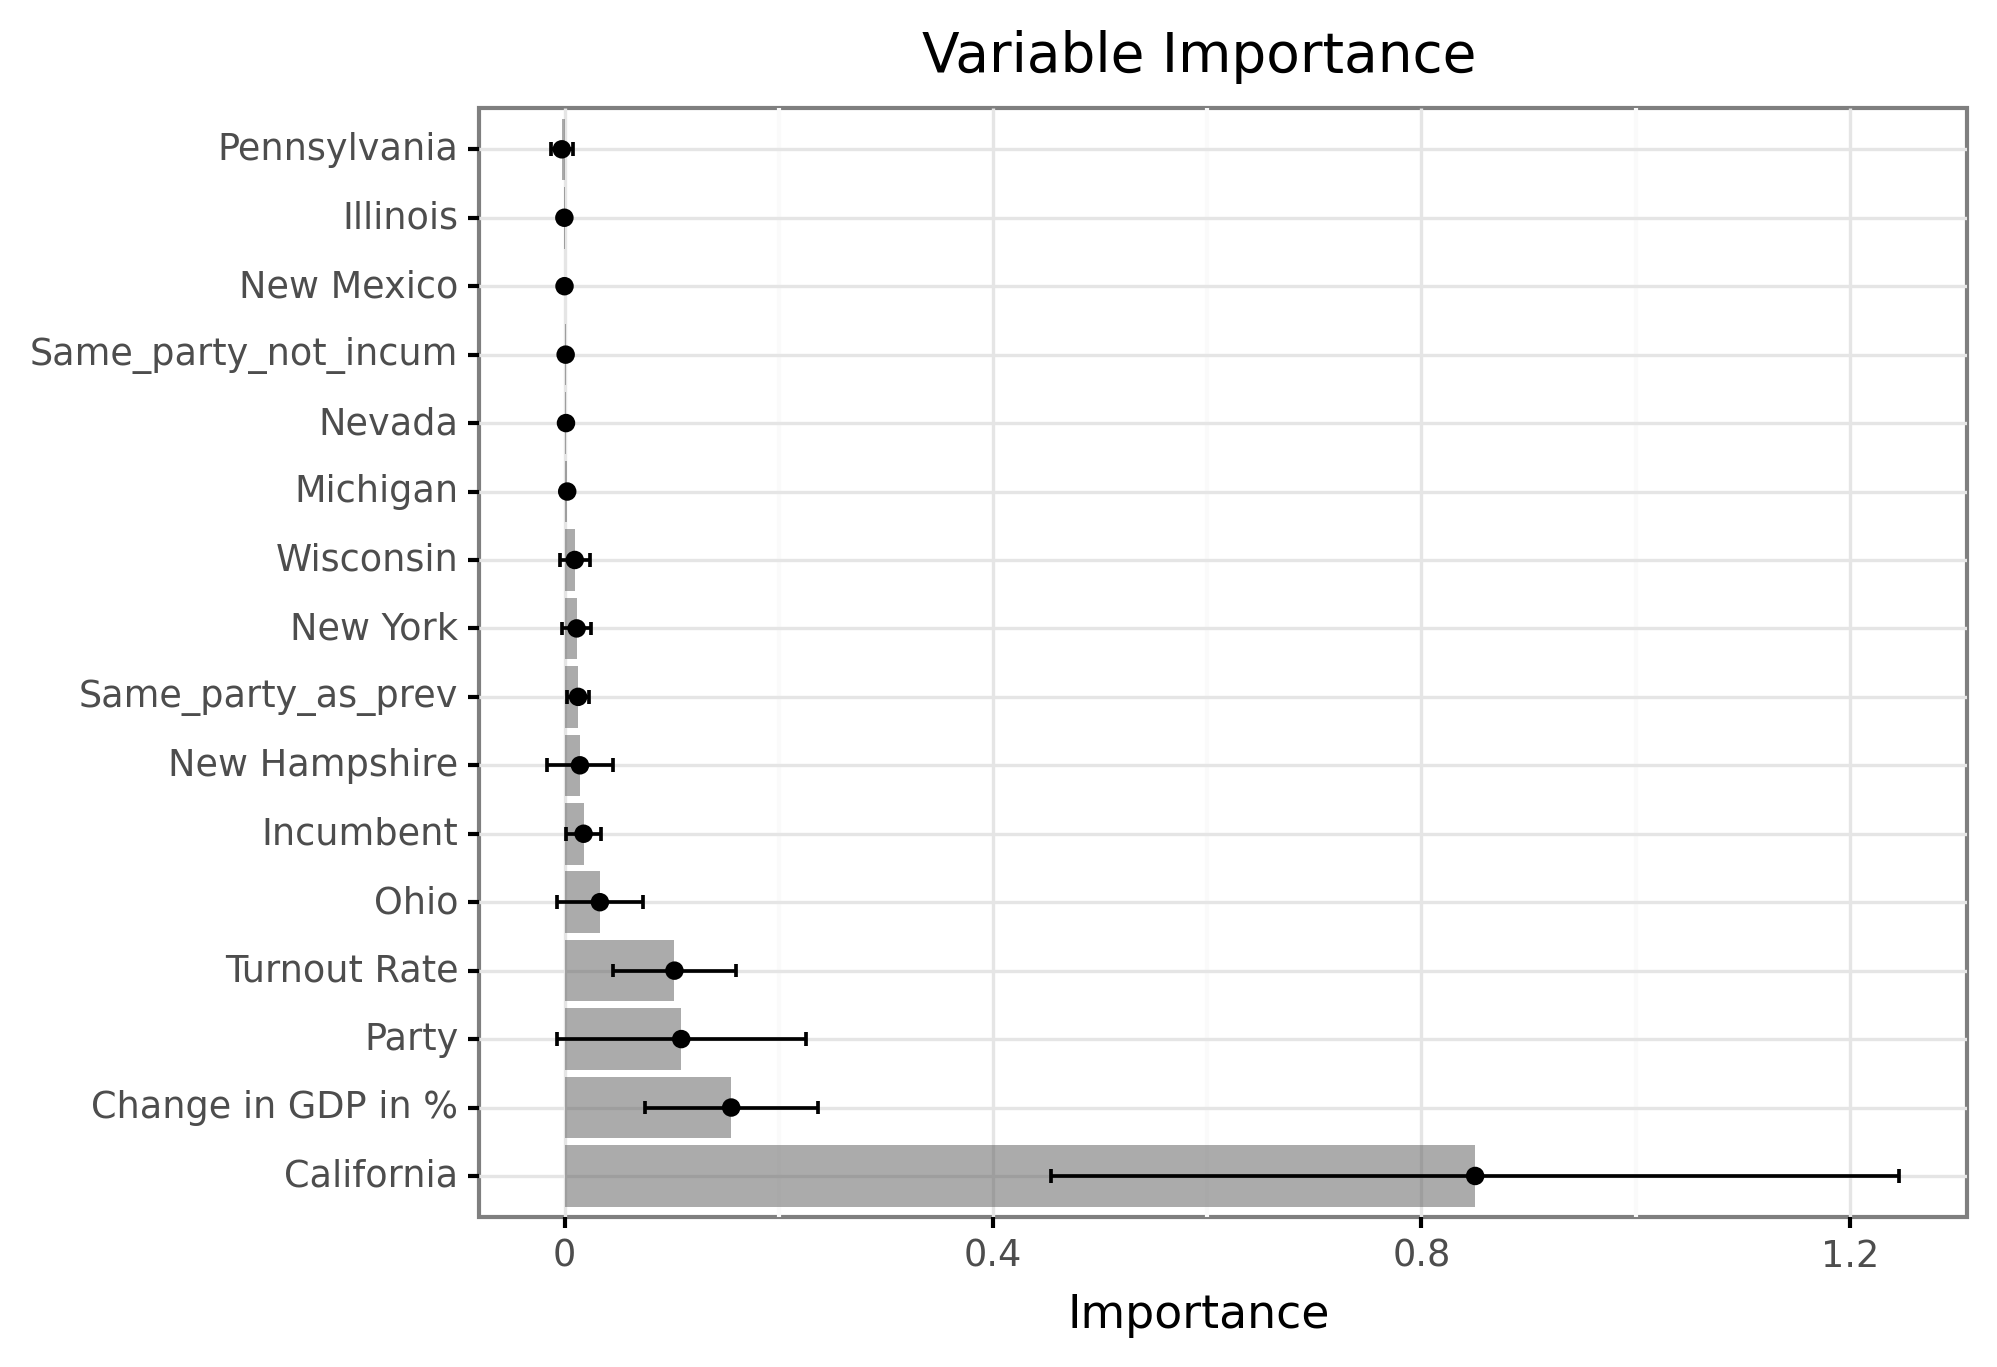
\includegraphics[width=0.7\linewidth]{variable_importance.png}
    \caption{Relative Variable Importance}
\end{figure}

Then, looking at the feature dependence plots below from the four most significant non-state features, there are some interesting effects. Party and Incumbent are both linear, but Change in GDP and Turnout Rate are a little more complex and somewhat quadratic. The effect of Change in GDP starts out relatively high for negative changes, and goes down some, with its lowest effects being at no change, which makes sense. Then, it goes up sharply - it has the greatest effects when there is a positive change in GDP. The maximum effect of Turnout Rate appears to be around 60. It's not quite as clear for this variable why this would be, but it would be an interesting thing to explore further. The effect of Incumbent being positive makes sense as we could see from the earlier graphs that there was a higher effect on Vote Share for incumbents than non-incumbents.

\begin{figure}[H]
    \centering
    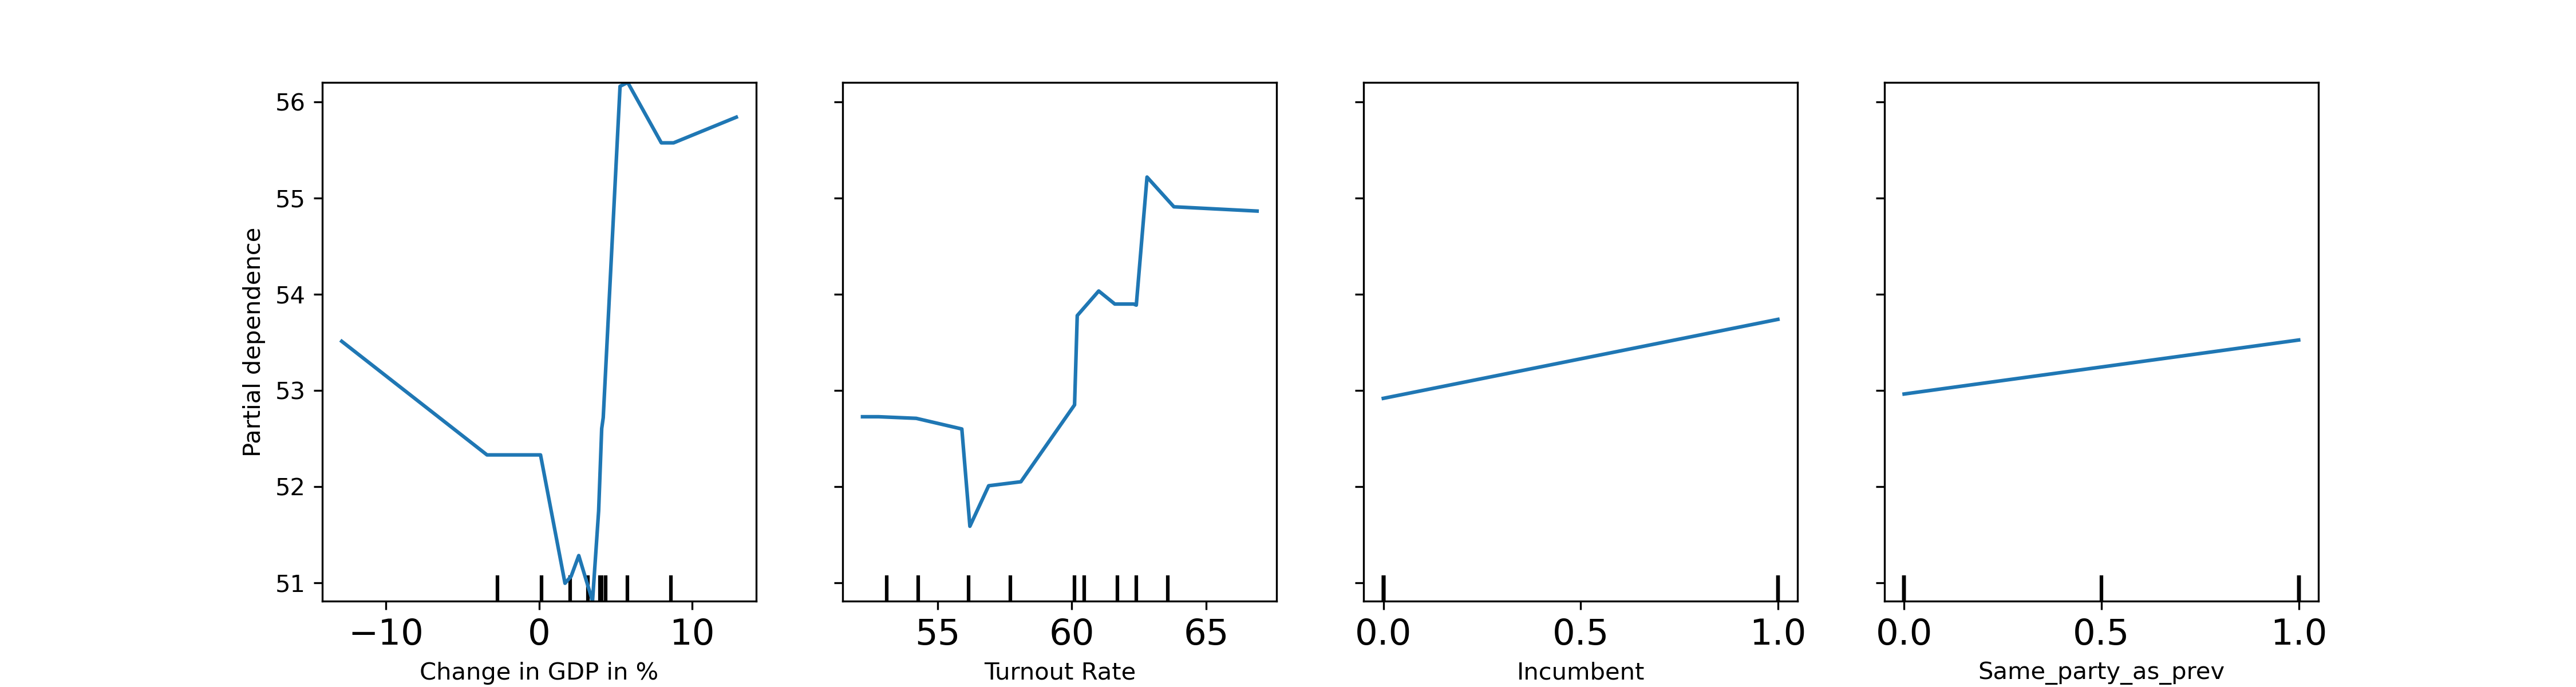
\includegraphics[width=0.9\linewidth]{Feature_dependence.png}
    \caption{Feature Dependence}
\end{figure}

\vspace{3.00mm}

\begin{figure}[H]
    \centering
    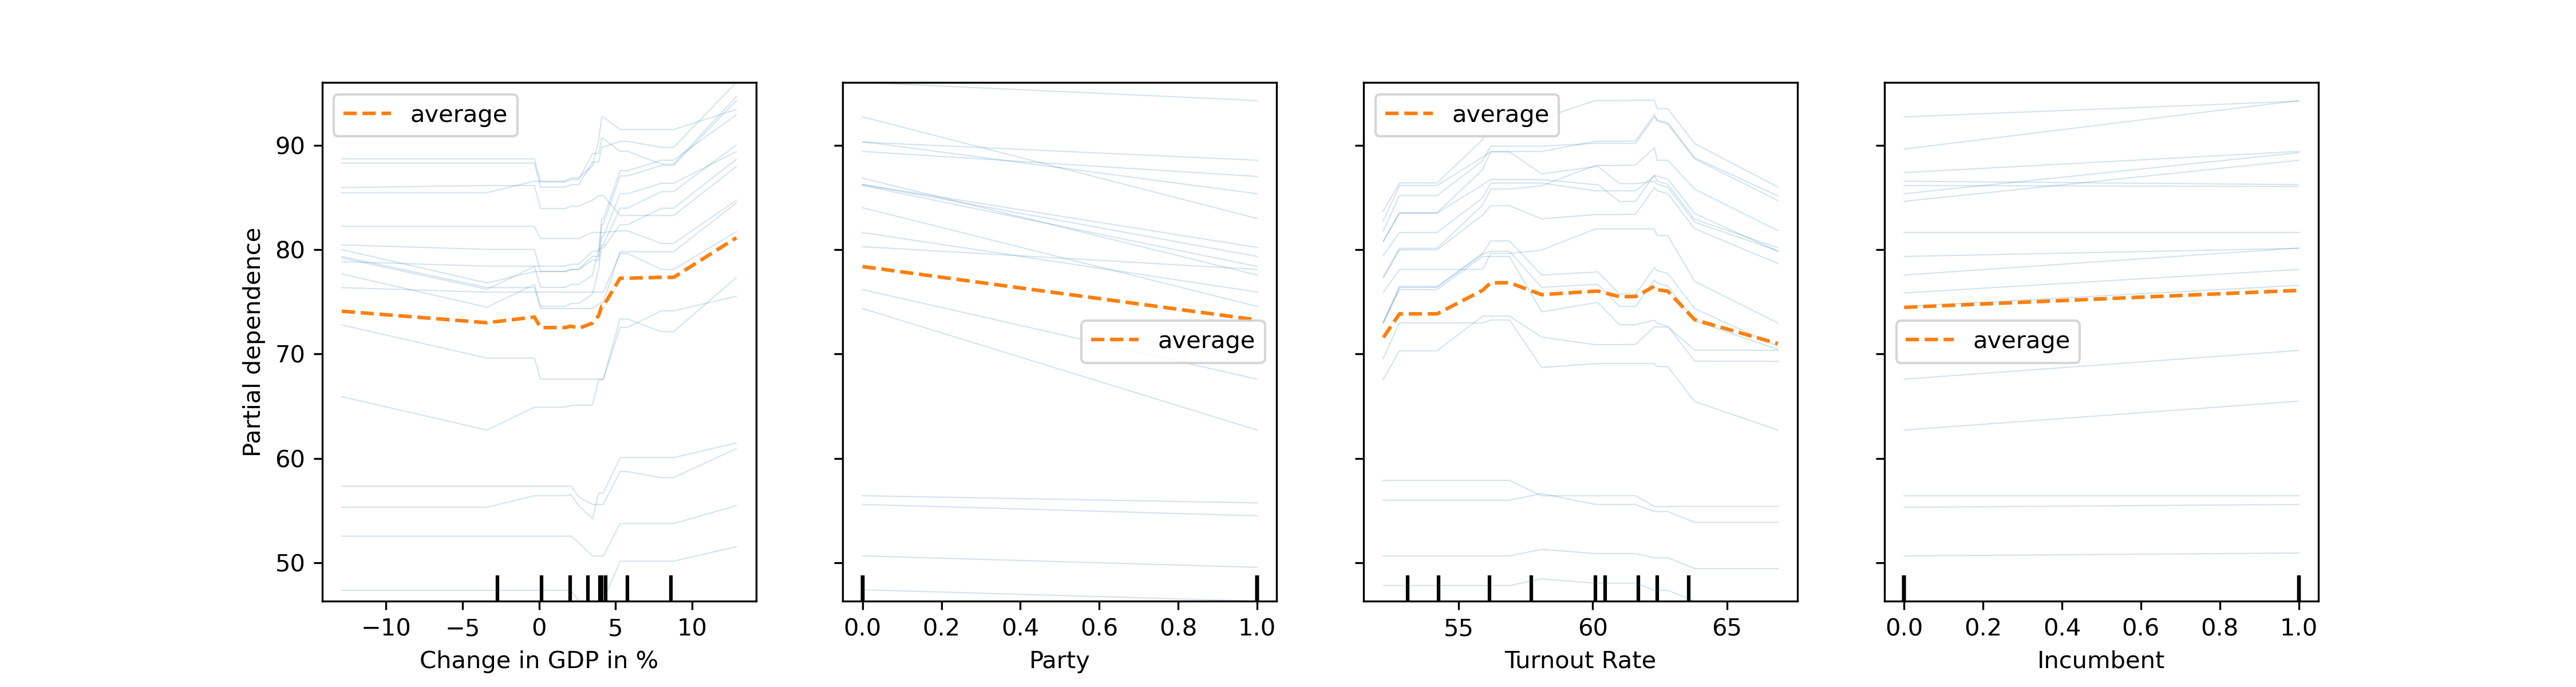
\includegraphics[width=0.9\linewidth]{ice_plot.png}
    \caption{Ice Plots}
\end{figure}

\section*{Discussion}

My project ended up being fairly successful, looking back on my original proposal. I was ultimately able to pull most of the data I wanted, organize it, and run a model. As I did have a very small sample size to run my analysis on, it made sense that my model was not the most predictive. The R-squared values being so low for the test data was very interesting - if I had more time, I would experiment with plotting out the relationship between the predicted values and the actual values to see if there are any clear patterns in the years that have the least accurate predicted values. It is possible that there are some patterns that have to do with the other features, or potentially are related to events from those years. 

\vspace{3.00mm}

The fact that the subset that included Change in GDP was potentially the most predictive was interesting to me - this suggests that, because there was only more recent data in this subset, there are more discernible patterns in recent years. This does make sense as the first several years in my data had a lot more variation, and so would be less able to add much to a predictive model. This would also be another interesting topic to explore further in the future.

\vspace{3.00mm}

I would also be interested in exploring the swing states in a slightly different way. My analysis of the swing states in the context of this project still included the other features, and I think it would be interesting to explore them on their own, or potentially see if I could find a more exact way to determine the most accurate swing states other than weighing the most recent ones differently.


\theendnotes
\end{document}

